\documentclass[12pt,a4paper]{article}
\usepackage{algorithm, algpseudocode, amsmath, amssymb, caption, csquotes, empheq, geometry, graphicx, hyperref, listings, multirow, physics, siunitx, subcaption, upgreek}
\usepackage[section]{placeins}

\title{Computational Physics\\Problem Set 3}
\author{Saleh Shamloo Ahmadi\\Student Number: 98100872}
\date{October 17, 2021}

\hypersetup{colorlinks=true, urlcolor=cyan}

\newcommand{\bdfig}{../fig/ballistic-deposition}
\newcommand{\pfig}{../fig/percolation}

\begin{document}
	\maketitle
    \section{Ballistic Deposition}
    Ballistic deposition models add particles randomly to a surface and in the case of non-random
    ballistic deposition models, apply specific rules after each "deposition".

    In general, we can approximately describe the growth of each model with the constants $\alpha$, $\beta$,
    and $z$ (not independent); If there is any interaction between neighboring points, the roughness of the
    surface (defined as the standard deviation of heights in one-dimensional systems) will approach an upper limit
    $w_s$ ($w(t)$ is the roughness) at \emph{time of saturation} $t_s$. Then
    \begin{gather}
        w(t) \sim t^\beta (\text{before saturation}), \\
        t_s \sim L^z, \quad w_s \sim L^\alpha \sim t_s^\beta \sim L^{z\beta},
    \end{gather}
    so we should have $\alpha = z\beta$. Note that depending on the method used to determine saturation time, $\beta$
    before saturation can be different form $\beta$ obtained from saturation.

    \subsection{Ballistic Deposition with Relaxation}
    In this model, after each deposition, the particle is dropped onto a neighboring point if it is at a lower height
    (less particles have been deposited on that point). If more than one neighbor has a lower height, the particle is
    dropped onto the point with the lowest height.

    The faint "bands" in each plot shows the standard deviation of each data point taken over all runs.
    \newgeometry{top=0.1in, bottom=1in}
    \begin{figure}
        \centering
        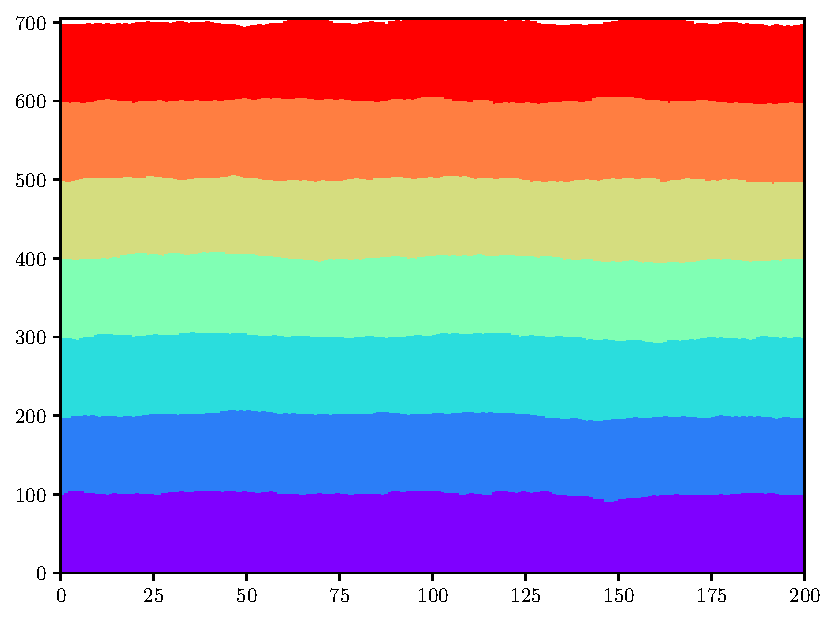
\includegraphics[width=\linewidth]{\bdfig/bd-relax-vis}
    \end{figure}
    \begin{figure}
        \centering
        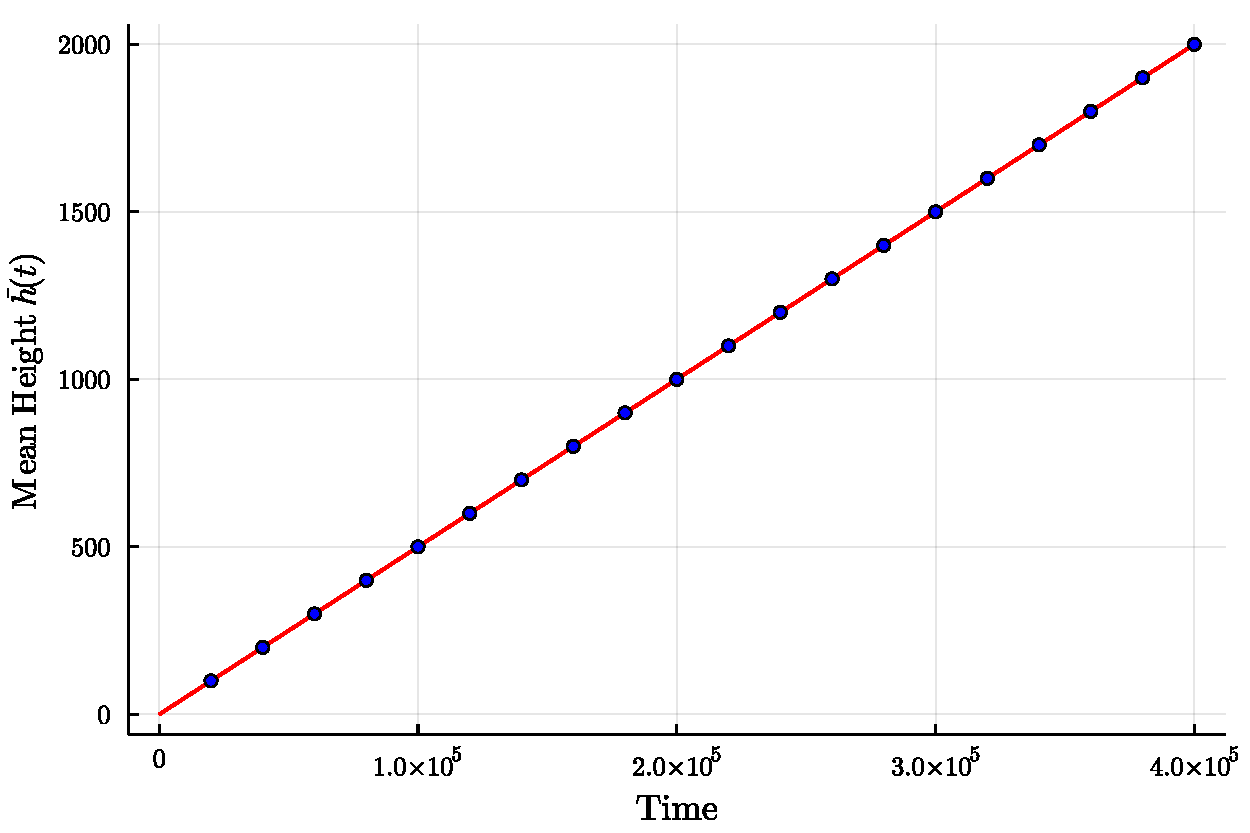
\includegraphics[width=\linewidth]{\bdfig/bd-relax-mean}
        \caption{$\text{slope}=0.005\pm\num{6e-20}$}
    \end{figure}
    \begin{figure}
        \centering
        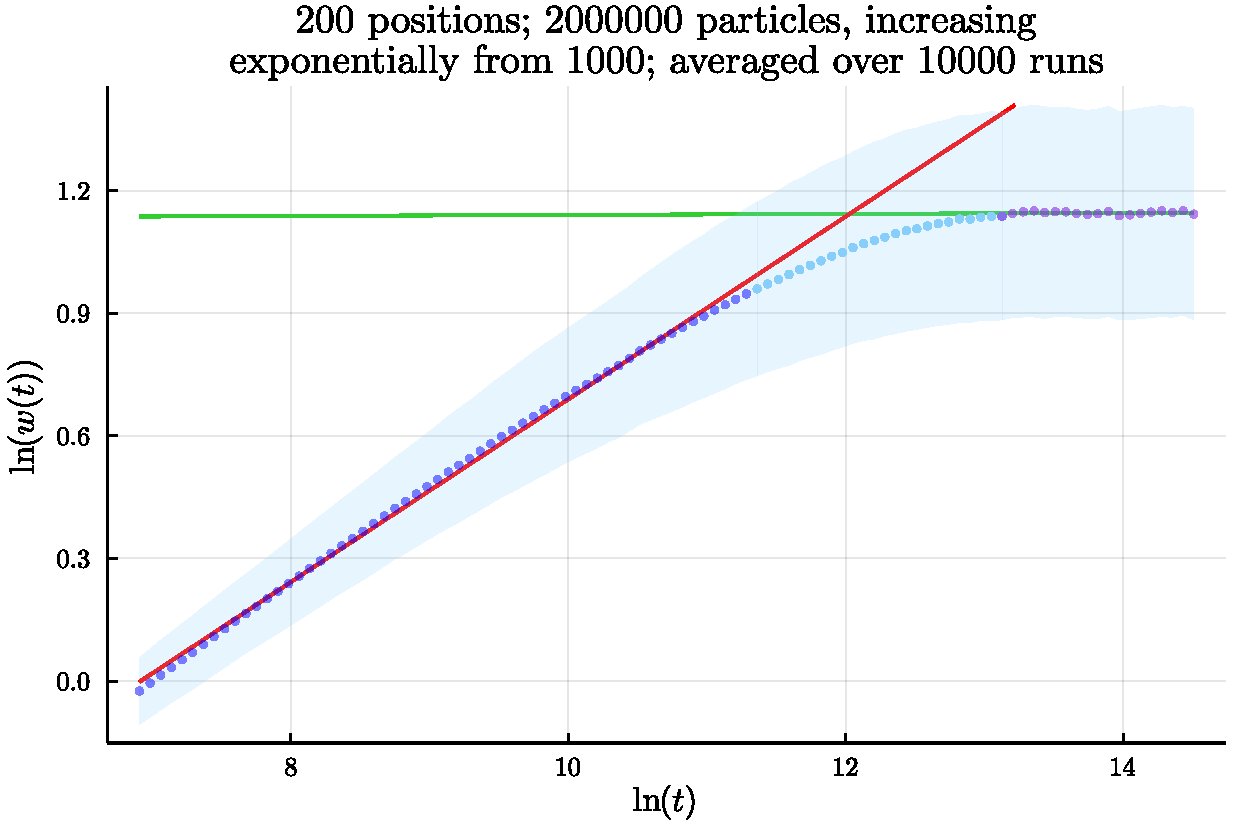
\includegraphics[width=\linewidth]{\bdfig/bd-relax-roughness-200}
        \caption{$\beta=0.224\pm0.001$}
    \end{figure}
    \begin{figure}
        \centering
        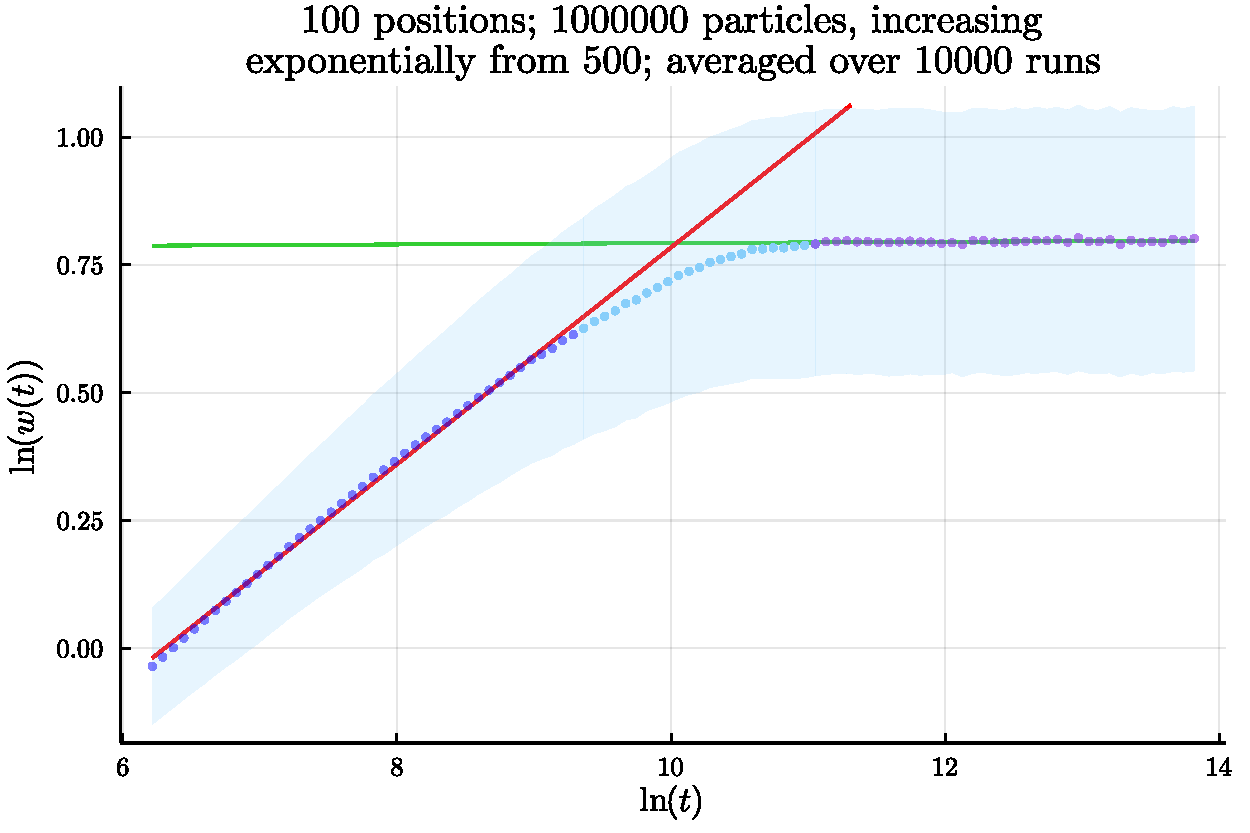
\includegraphics[width=\linewidth]{\bdfig/bd-relax-roughness-100}
    \end{figure}
    \begin{figure}
        \centering
        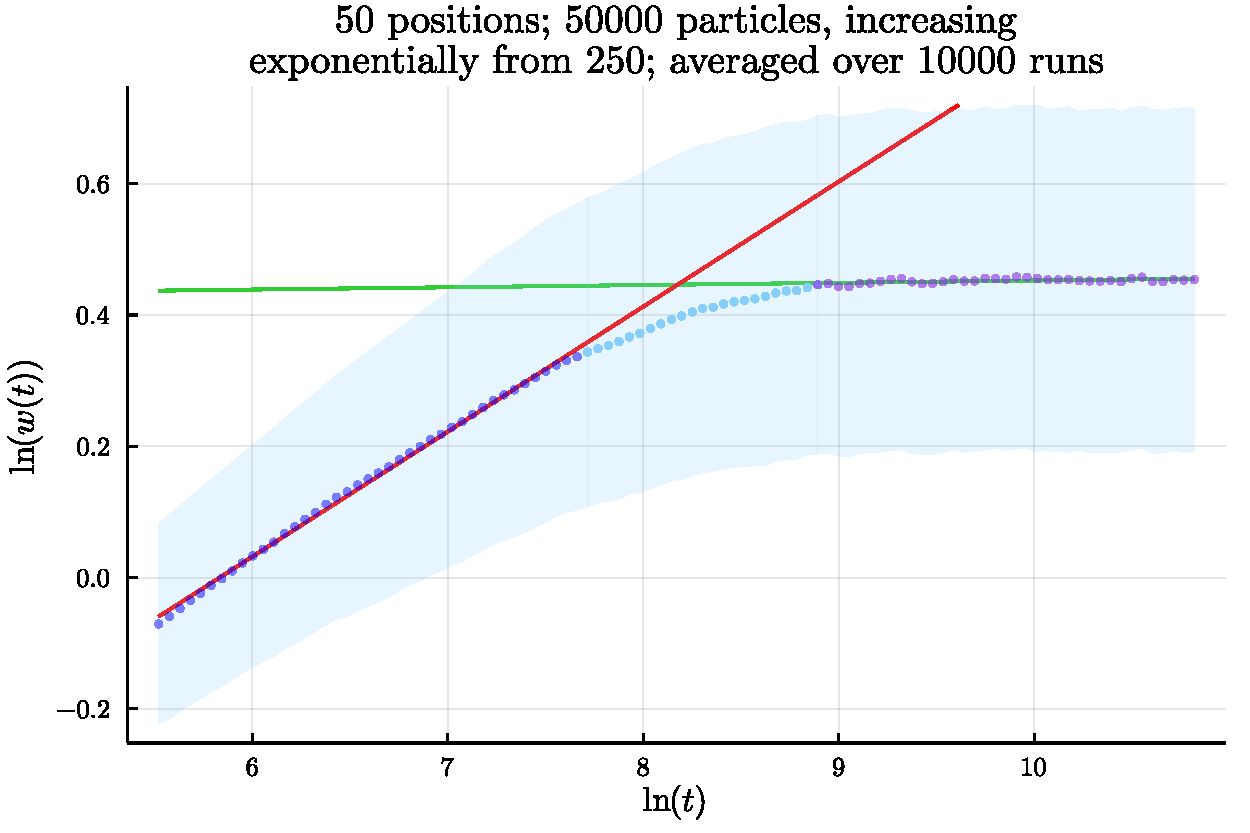
\includegraphics[width=\linewidth]{\bdfig/bd-relax-roughness-50}
    \end{figure}
    \begin{figure}
        \centering
        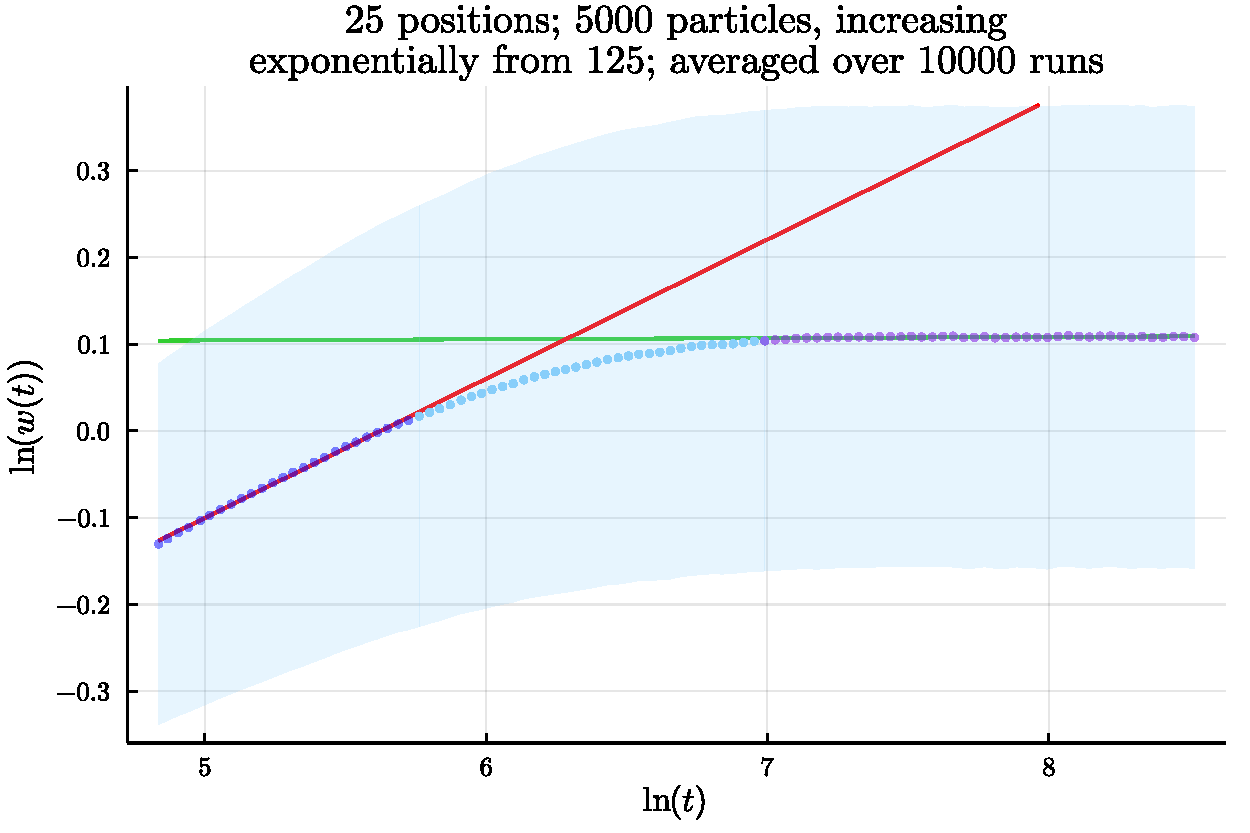
\includegraphics[width=\linewidth]{\bdfig/bd-relax-roughness-25}
    \end{figure}
    \begin{figure}
        \centering
        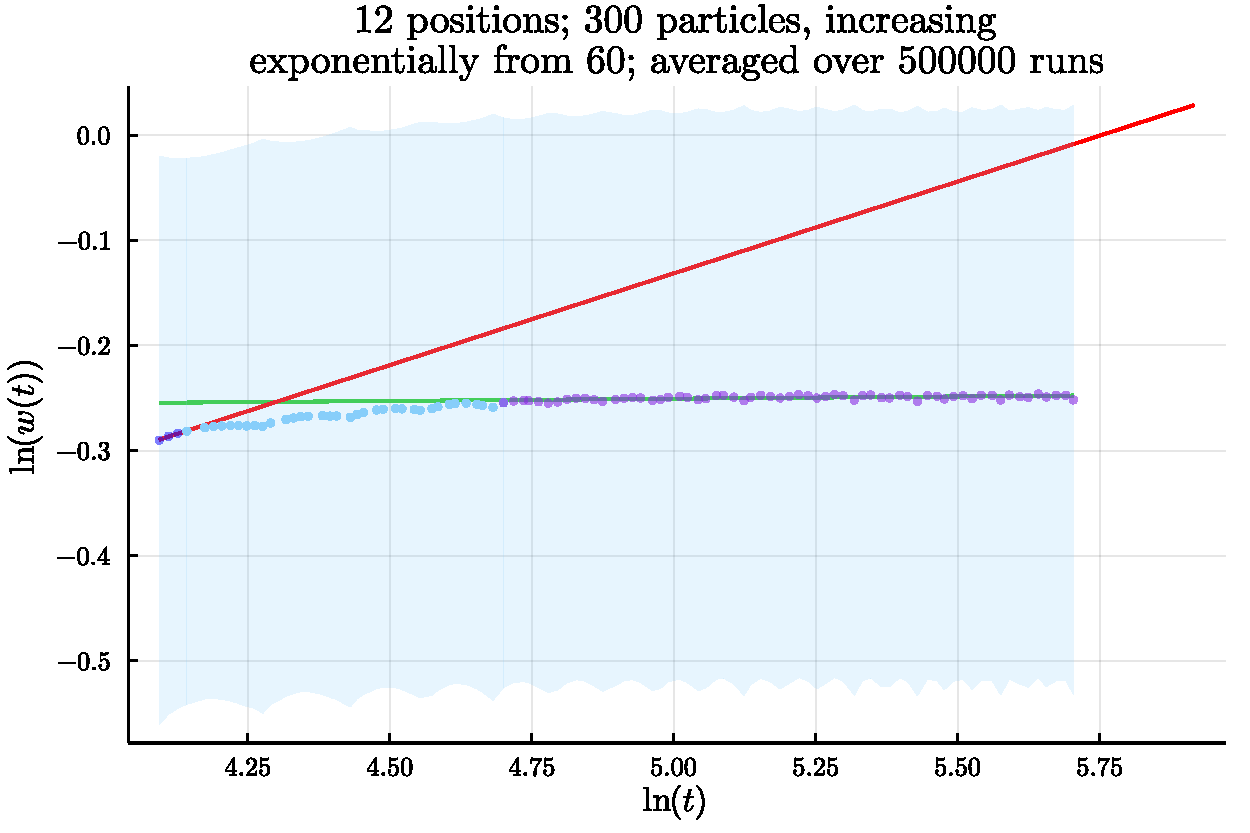
\includegraphics[width=\linewidth]{\bdfig/bd-relax-roughness-12}
    \end{figure}
    \begin{figure}
        \centering
        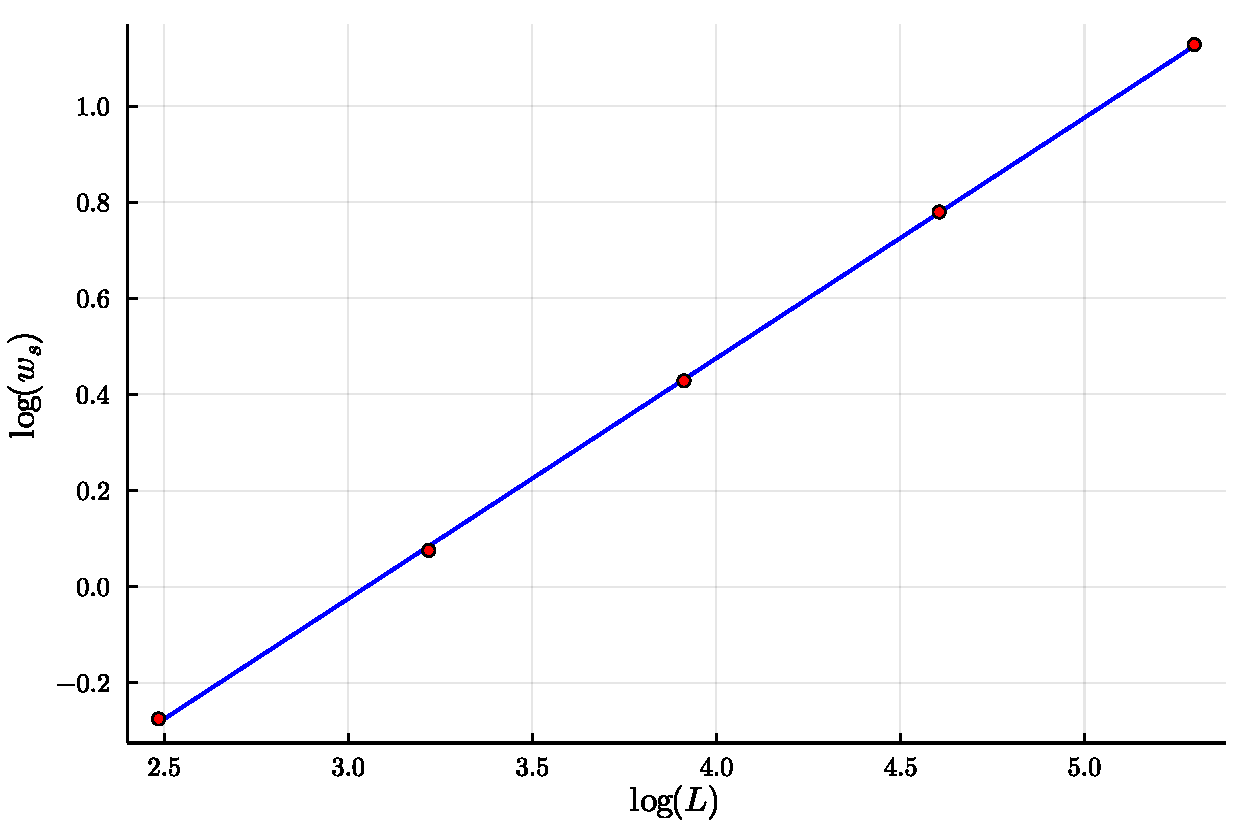
\includegraphics[width=\linewidth]{\bdfig/bd-relax-sat-alpha}
        \caption{$\alpha = 0.500\pm0.003$}
    \end{figure}
    \begin{figure}
        \centering
        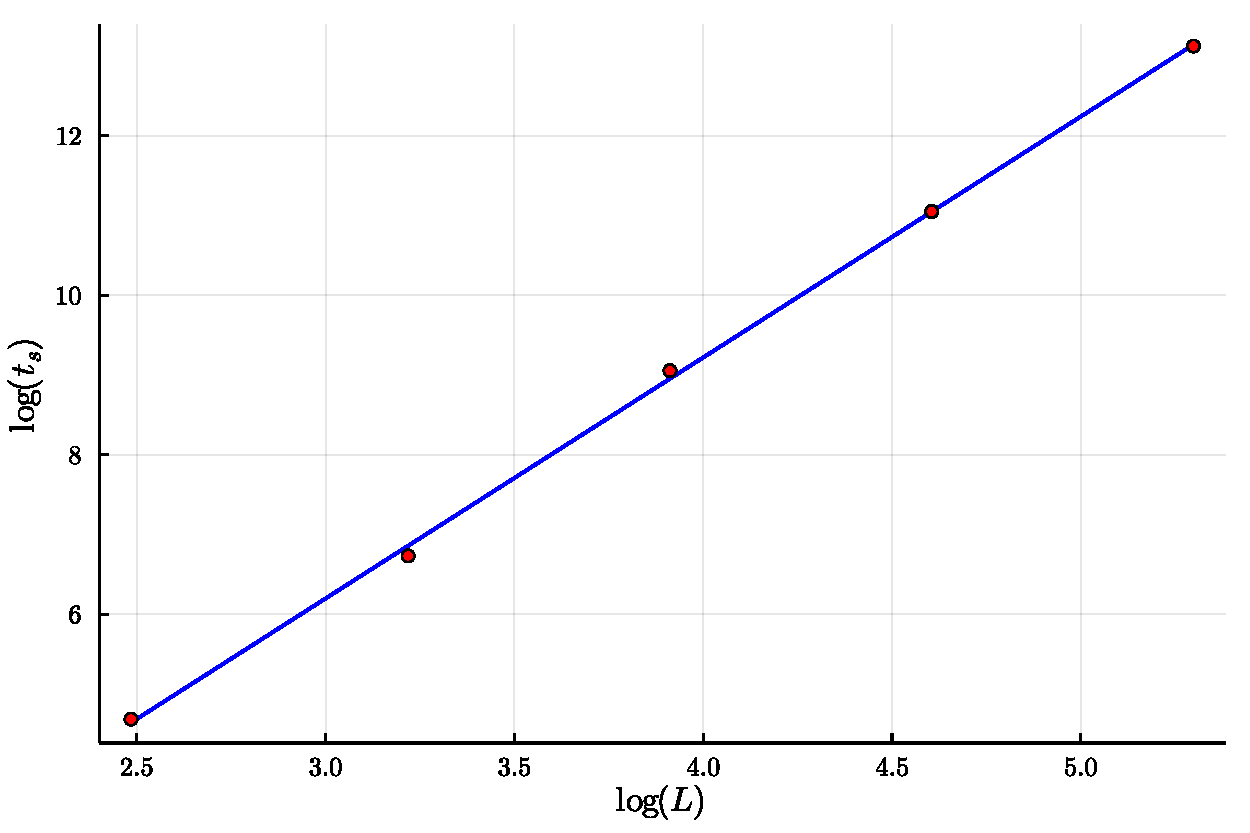
\includegraphics[width=\linewidth]{\bdfig/bd-relax-sat-z}
        \caption{$z = 3.02\pm0.04$}
    \end{figure}
    \begin{figure}
        \centering
        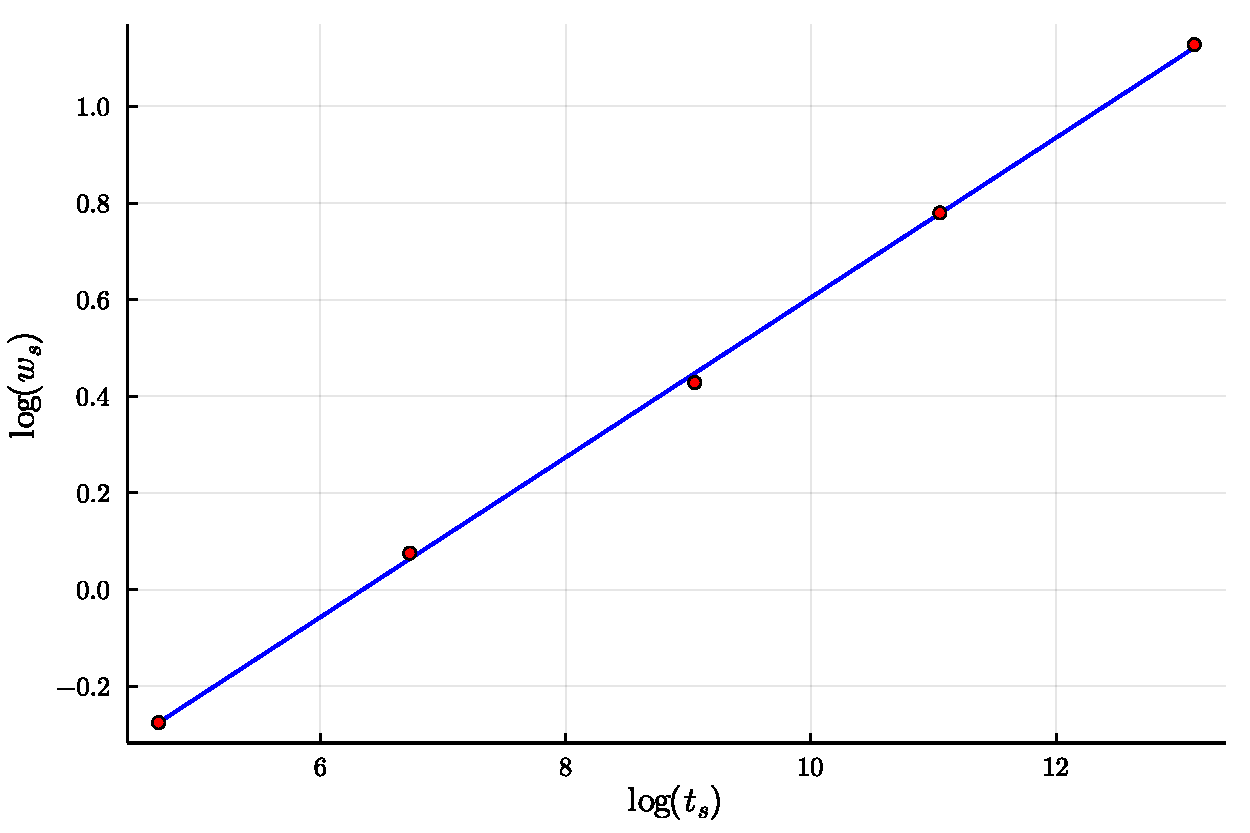
\includegraphics[width=\linewidth]{\bdfig/bd-relax-sat-beta}
        \caption{$\beta = 0.165\pm0.002$}
    \end{figure}
    \restoregeometry
    \begin{table}[htb!]
        \centering
        \caption{Ballistic Deposition with Relaxation}
        \begin{tabular}{|c|c|c|}
            \hline
            $L$ & $t_s$ & $w_s$ \\
            \hline
            12 & 108 & 0.759364 \\
            \hline
            25 & 837 & 1.07834 \\
            \hline
            50 & 8550 & 1.53467 \\
            \hline
            100 & 63042 & 2.18055 \\
            \hline
            200 & 502161 & 3.08905 \\
            \hline
        \end{tabular}
    \end{table}
    I calculated the time of saturation by fitting a line through the trailing points with constant $w(t)$.
    This method is not optimal. It would be better to find the intersection of the linear fit and constant fit lines.
    Due to a lack of time, I am unfortunately stuck with this (this was the first method I tried and there was no time
    left before the deadline to improve my methodology).

    As you can see, this description of the model is not perfect, since $\beta$ is not the same as $L$ changes.
    \subsection{Ballistic Deposition (regular)}
    In this model, particles stick to the first point they come in contact with. This means each particle will be stuck
    at the maximum heigh in its dropping neighborhood
    ($\text{max}\{h_{\text{left}}, h_{\text{drop}} + 1, h_{\text{right}}\}$).

    Results have similar characteristics to the last model. Notably, $\beta$ obtained from saturation is equal
    within the margin of error and $\beta$ obtained from ftting to data is also very close. $\alpha$ and $z$ are
    smaller, since correlation is stronger in this model (height of each point is directly related to the neighboring
    heights, instead of being indirectly affected by them through the distribution of heights).
    \begin{table}[hbt!]
        \centering
        \caption{Ballistic Deposition (regular)}
        \begin{tabular}{|c|c|c|}
            \hline
            $L$ & $t_s$ & $w_s$ \\
            \hline
            12 & 107 & 2.42859 \\
            \hline
            25 & 406 & 2.84437 \\
            \hline
            50 & 2715 & 4.20796 \\
            \hline
            100 & 12386 & 4.94841 \\
            \hline
            200 & 65003 & 6.75316 \\
            \hline
        \end{tabular}
    \end{table}
    \newgeometry{top=0.1in, bottom=1in}
    \begin{figure}
        \centering
        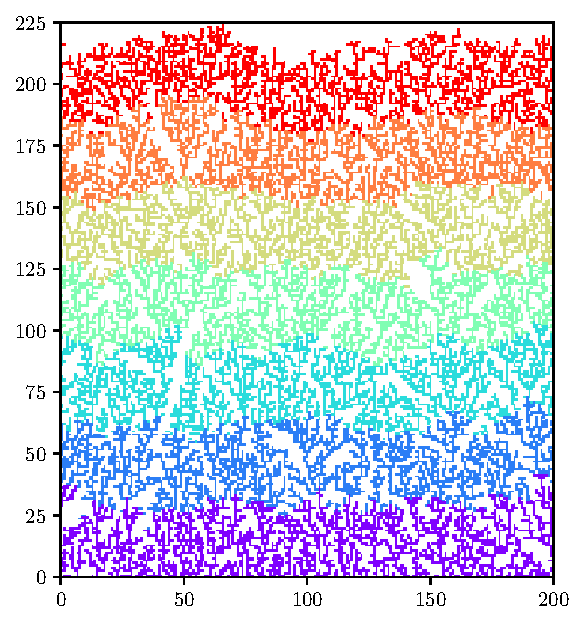
\includegraphics[width=\linewidth]{\bdfig/bd-vis}
    \end{figure}
    \begin{figure}
        \centering
        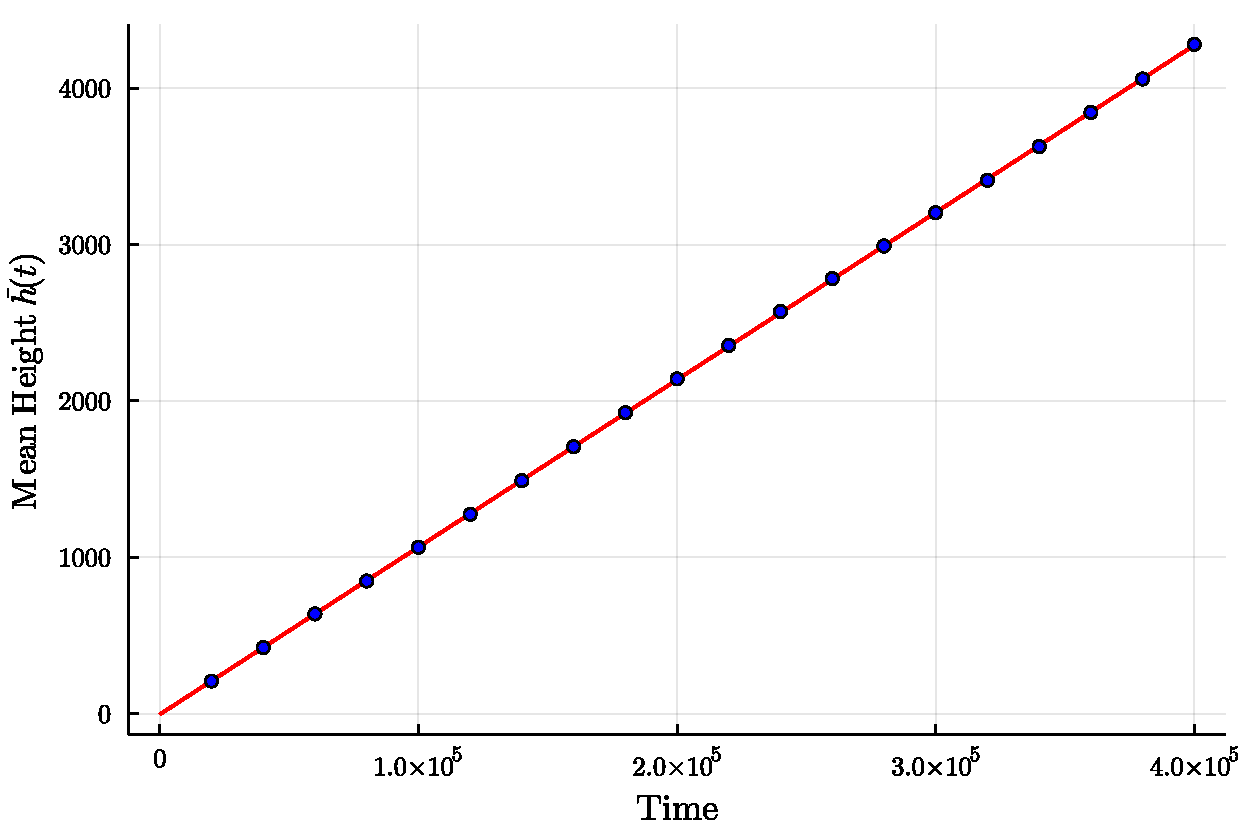
\includegraphics[width=\linewidth]{\bdfig/bd-mean}
        \caption{$\text{slope}=\num{1.0698e-2}\pm\num{9e-6}$}
    \end{figure}
    \begin{figure}
        \centering
        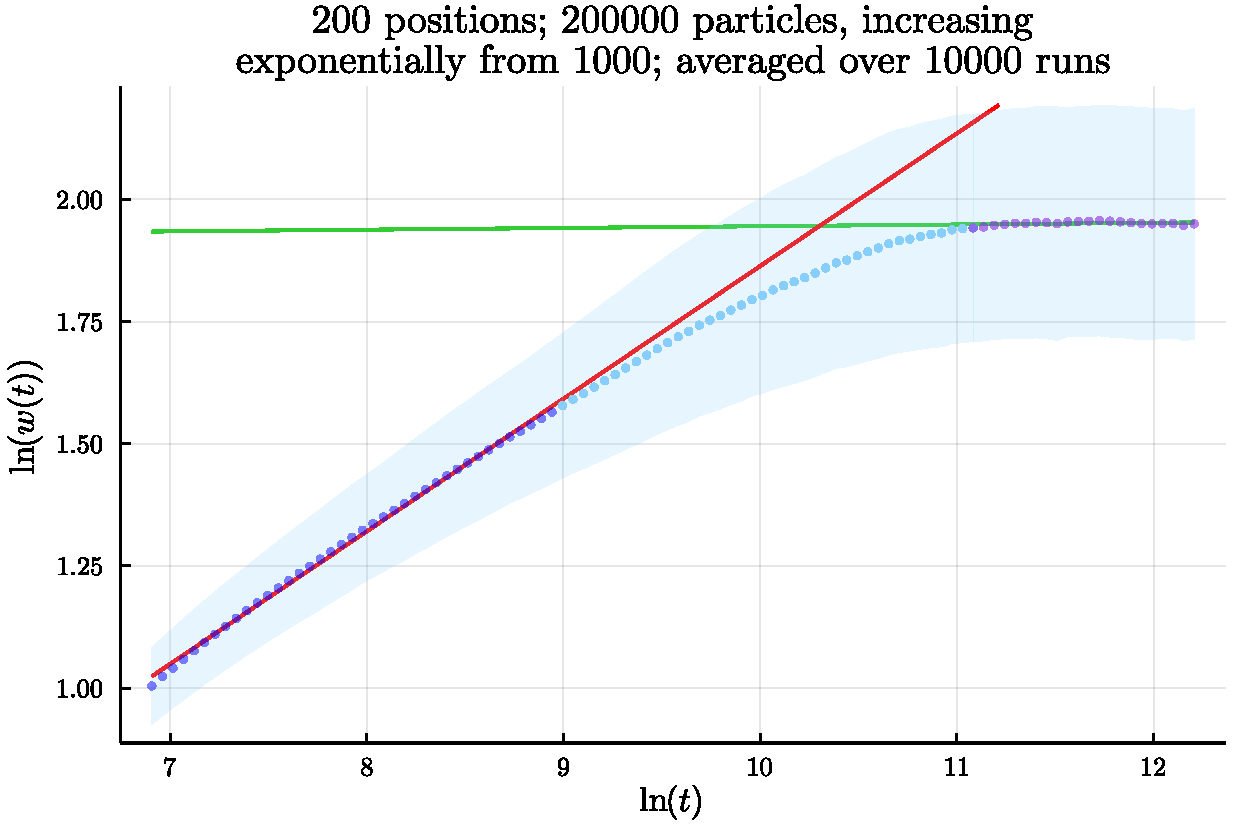
\includegraphics[width=\linewidth]{\bdfig/bd-roughness-200}
    \end{figure}
    \begin{figure}
        \centering
        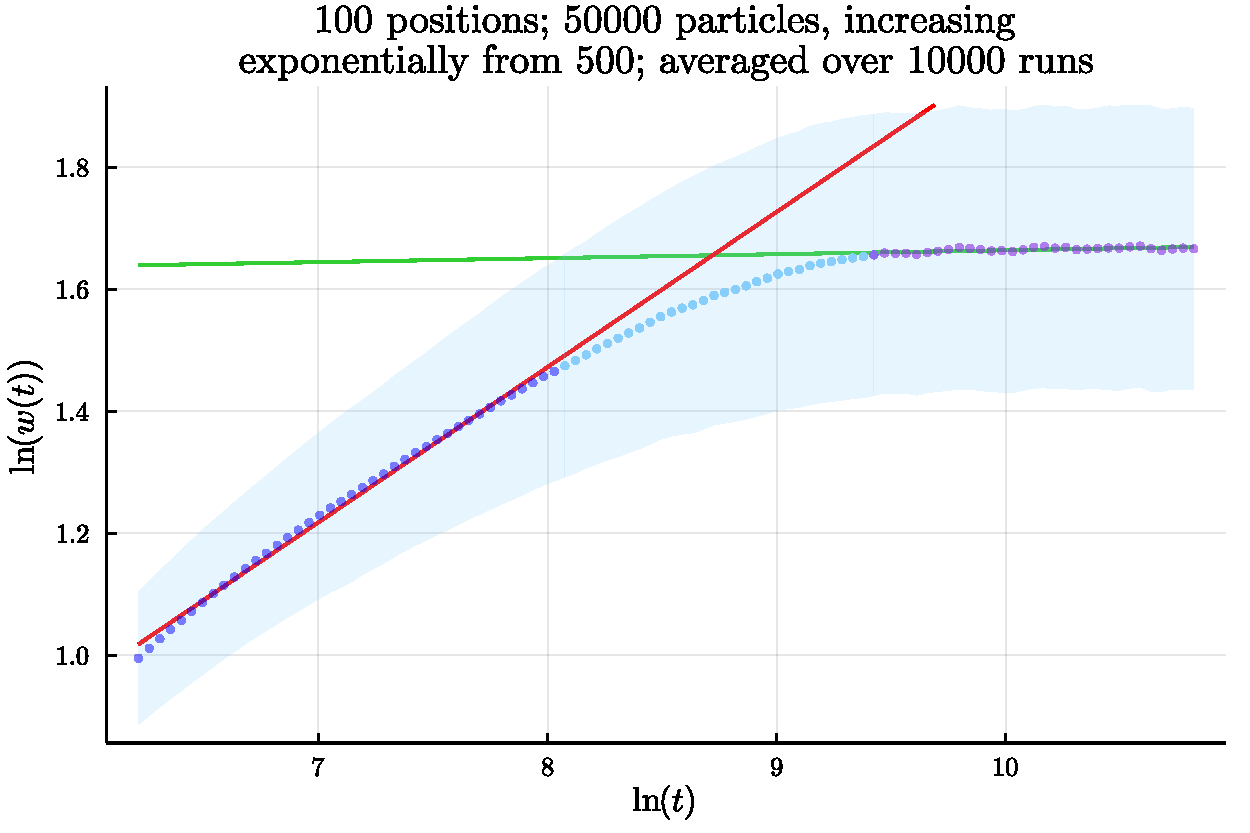
\includegraphics[width=\linewidth]{\bdfig/bd-roughness-100}
        \caption{$\beta=0.254\pm0.003$}
    \end{figure}
    \begin{figure}
        \centering
        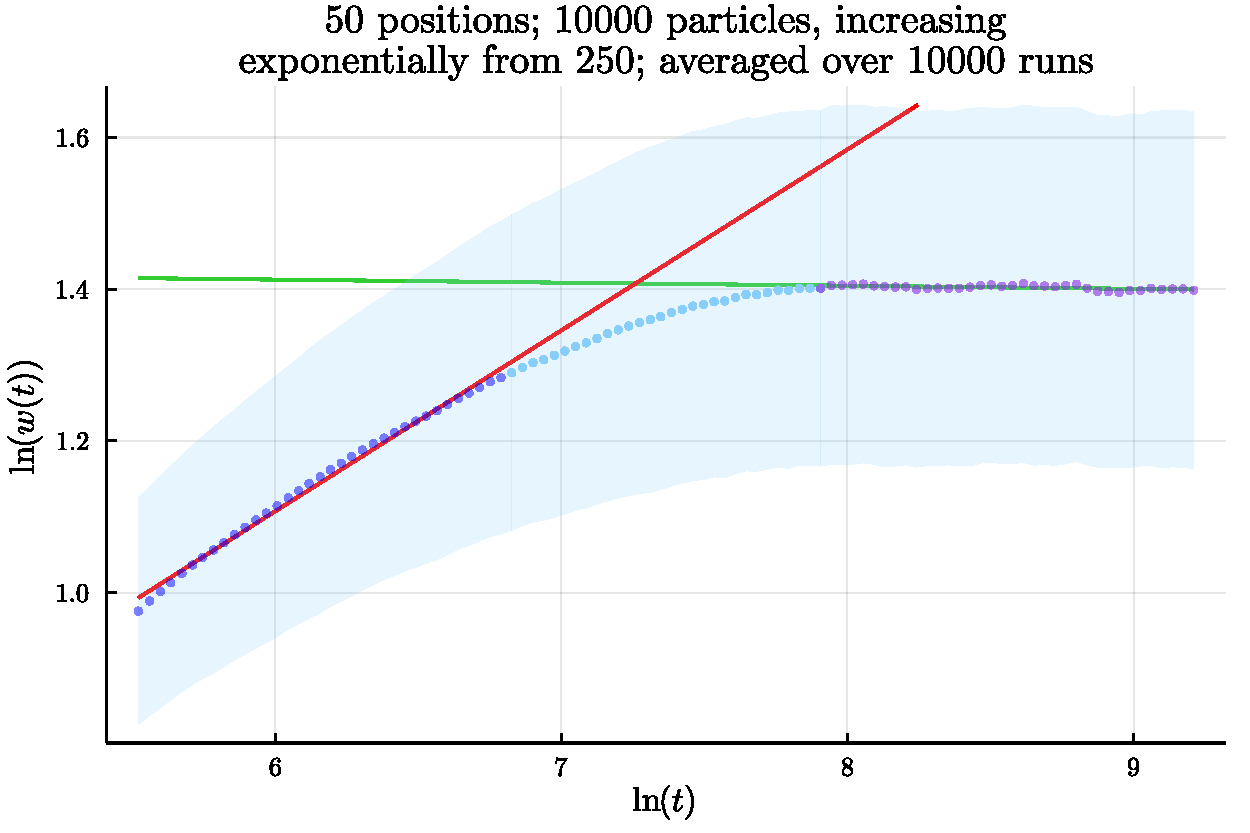
\includegraphics[width=\linewidth]{\bdfig/bd-roughness-50}
    \end{figure}
    \begin{figure}
        \centering
        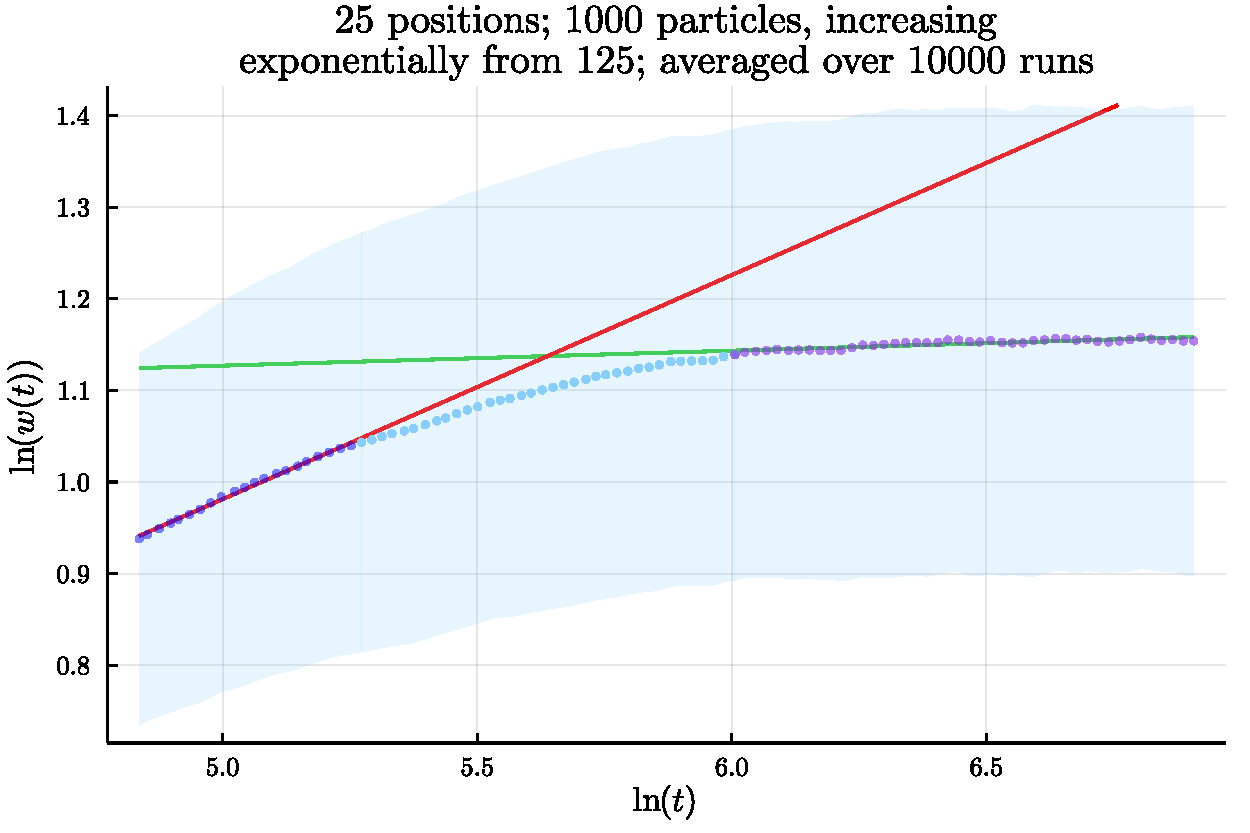
\includegraphics[width=\linewidth]{\bdfig/bd-roughness-25}
    \end{figure}
    \begin{figure}
        \centering
        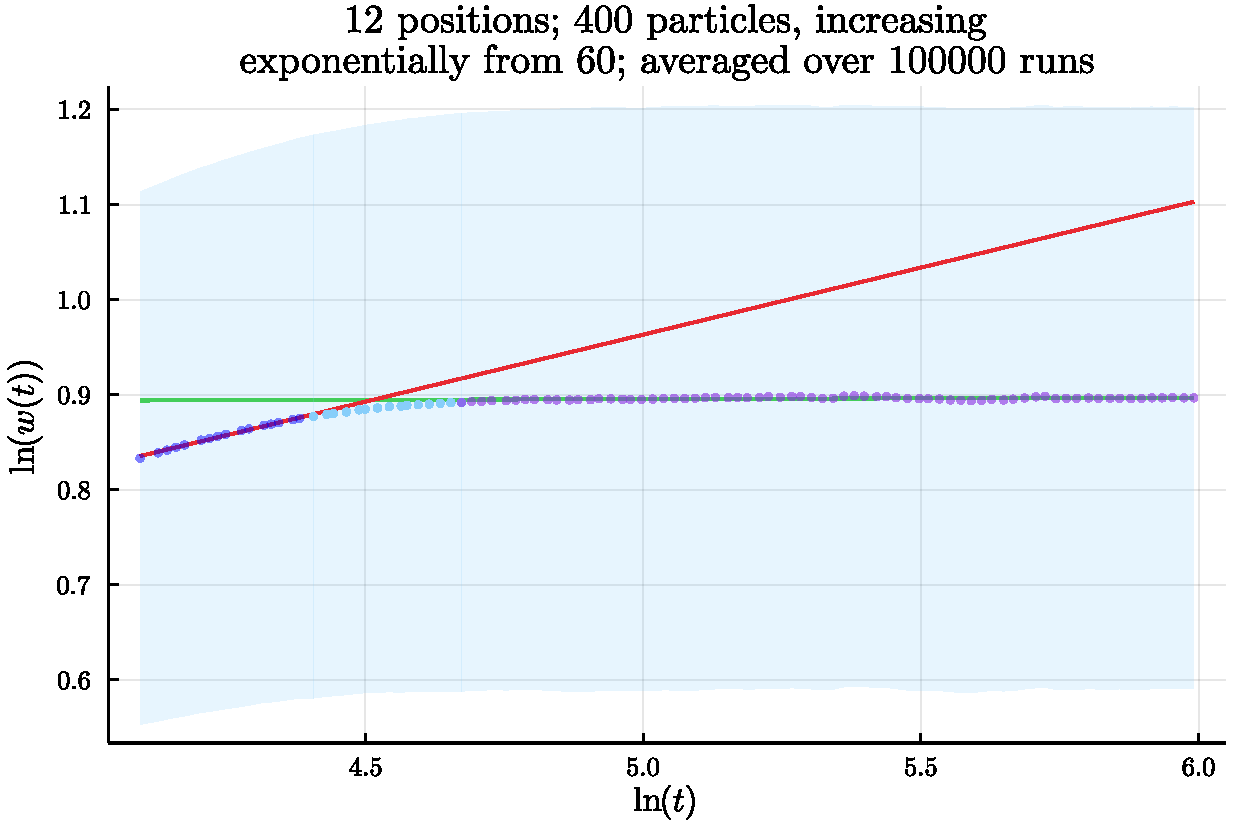
\includegraphics[width=\linewidth]{\bdfig/bd-roughness-12}
    \end{figure}
    \begin{figure}
        \centering
        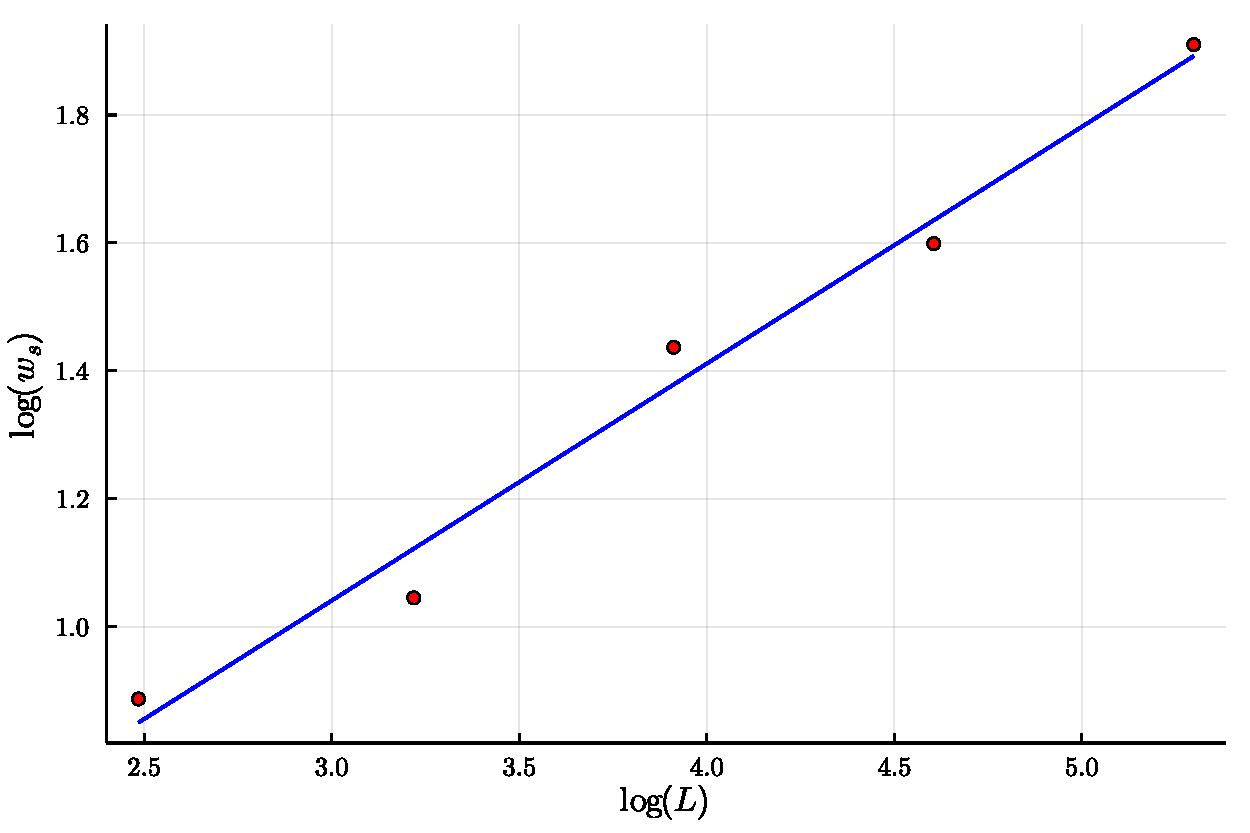
\includegraphics[width=\linewidth]{\bdfig/bd-sat-alpha}
        \caption{$\alpha = 0.37\pm0.03$}
    \end{figure}
    \begin{figure}
        \centering
        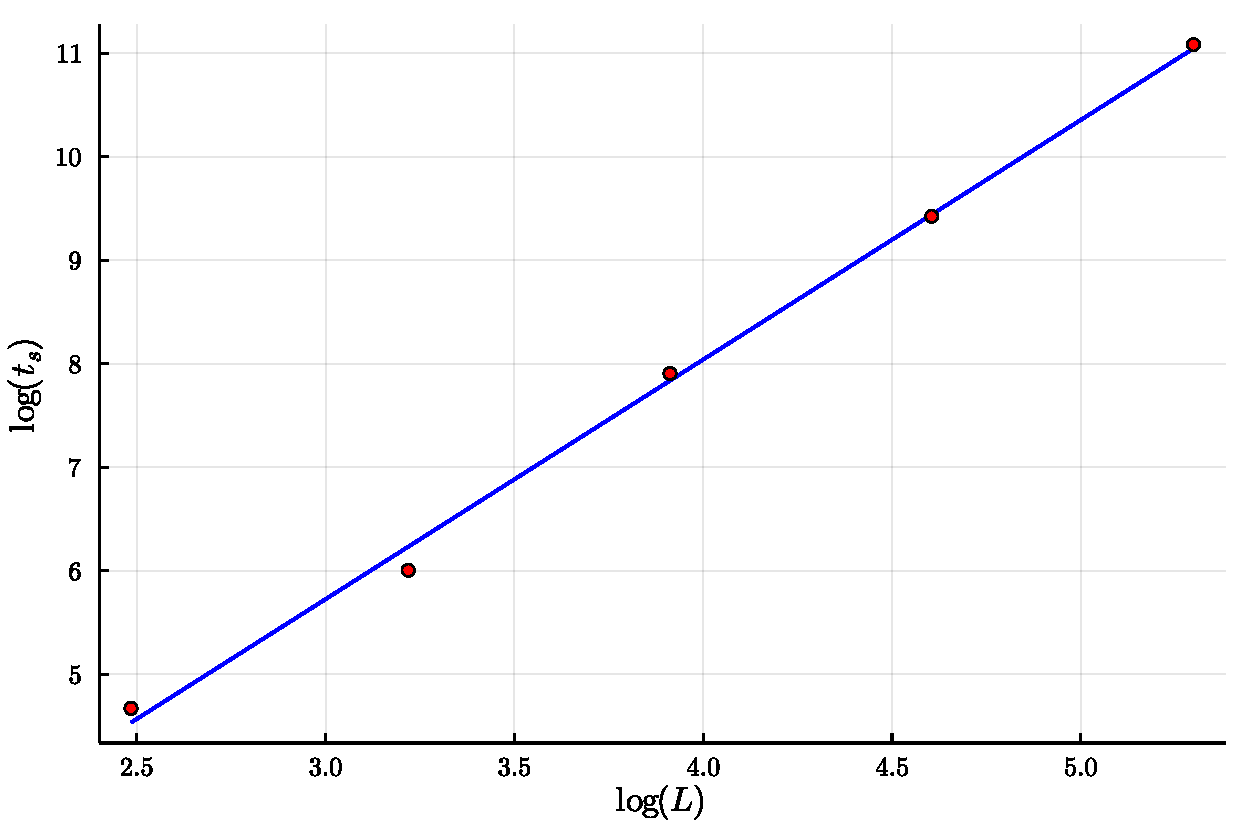
\includegraphics[width=\linewidth]{\bdfig/bd-sat-z}
        \caption{$z = 2.31\pm0.07$}
    \end{figure}
    \begin{figure}
        \centering
        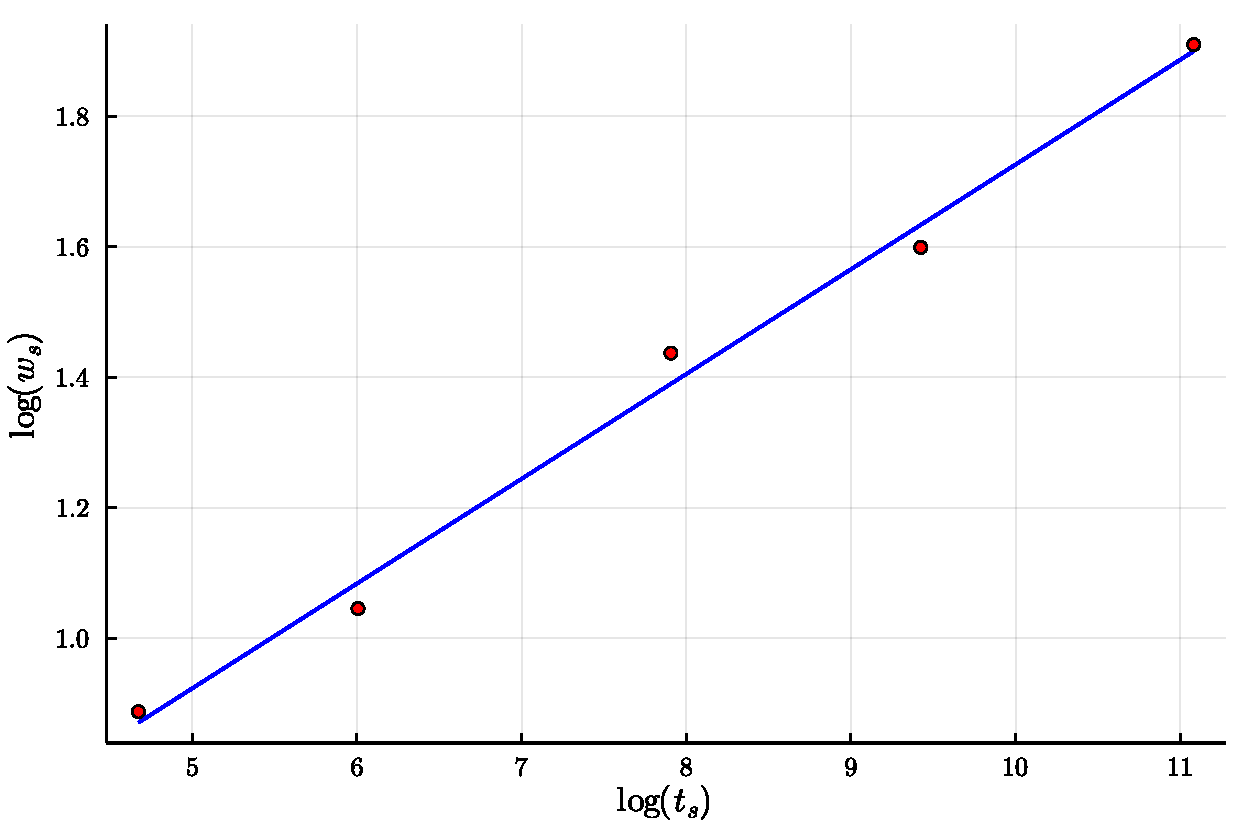
\includegraphics[width=\linewidth]{\bdfig/bd-sat-beta}
        \caption{$\beta = 0.161\pm0.008$}
    \end{figure}
    \restoregeometry
    \subsubsection{Correlation Length}
    In the ballistic deposition model, each point can have long range effect on further points through clustering with
    its neighbors, which in turn cluster with their own neighbors, and so on. To find the range of interaction, or
    \emph{the correlation length}, we can isolate the particles that stem from a single point
    (the "tree" attached to a "seed).
    \begin{figure}
        \centering
        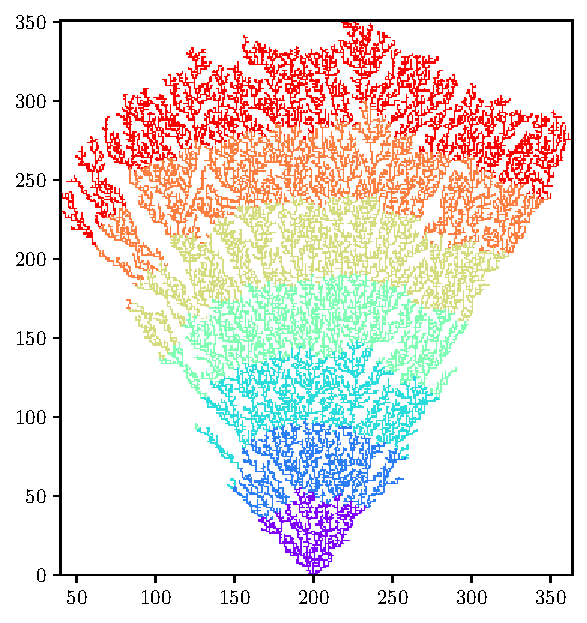
\includegraphics[width=\linewidth]{\bdfig/bd-iso-vis}
    \end{figure}
    \begin{figure}
        \centering
        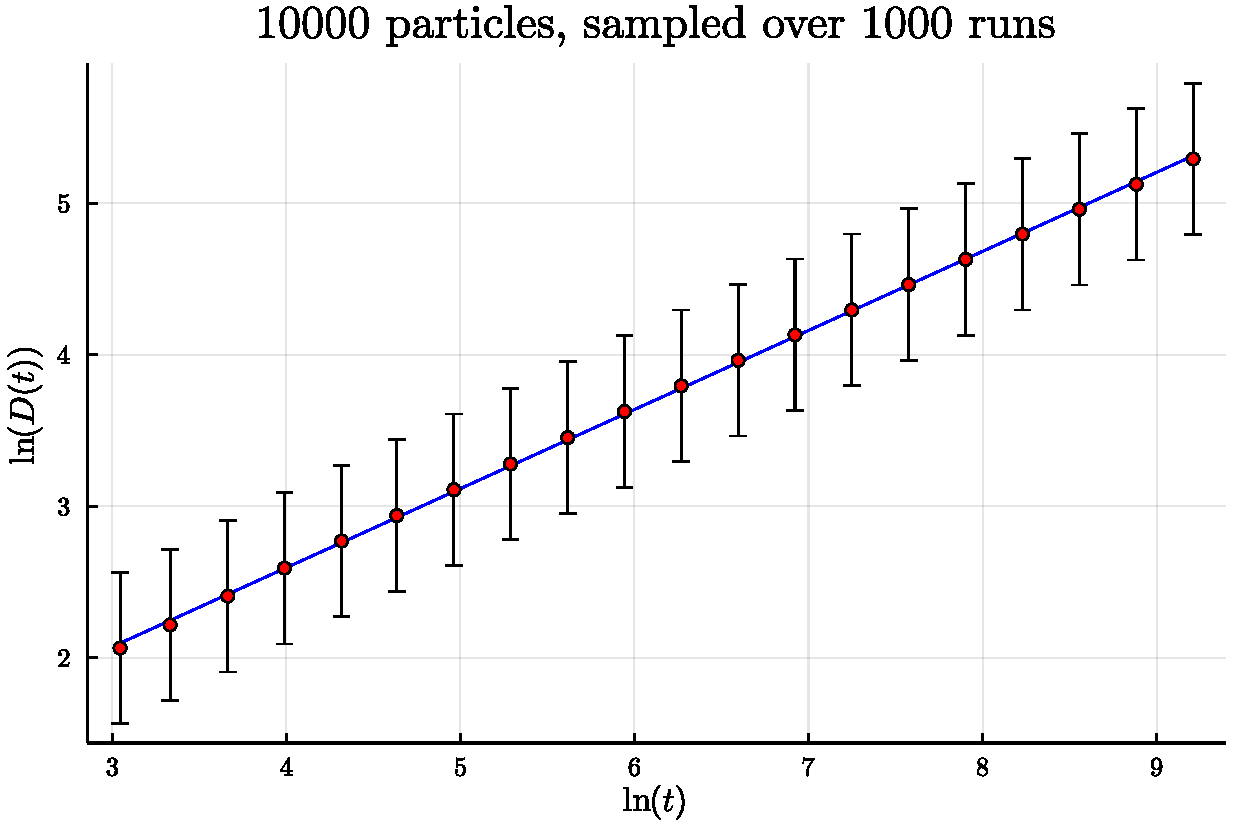
\includegraphics[width=\linewidth]{\bdfig/bd-correlation}
        \caption{$\text{slope} = 0.522\pm0.002$.\\The slope is the growth exponent for of the correlation length.}
    \end{figure}
    \section{Percolation}
    \subsection{Depth-First Search}
    Using a modified version of the depth-first search algorithm (a.k.a. DFS) that is designed and optimized for grids,
    percolation problems can be solved efficiently (time complexity $\mathcal{O}(L^d)$, where L is the lenght
    of the grid and d is the number of dimentions). Algorithm \ref{alg:dfs} outlines the implementation.
    \begin{algorithm}
        \caption{DFS for solving a percolation problem}
        \label{alg:dfs}
        \begin{algorithmic}[1]
            \Function{DFS}{$G$} 
            \parbox[t]{0.75\linewidth}{\Comment{G is a boolean graph representing the empty/full states
            of each cell of the grid}}
                \State make stack $S$
                \ForAll{vertices $v$ \textbf{in} the starting row/column of the grid}
                    \If{$v$ \textbf{is} \textit{true}}
                        \State $S.push(v)$
                        \While{$S$ is not empty}
                            \State v = $S.pop()$
                            \If{$v$ is in the final row/column}
                                \State \textbf{return} \textit{true}
                            \ElsIf{$v$ is not already visited}
                                \State mark $v$ as visited
                                \ForAll{$w$ \textbf{in} $G.neighbors(v)$}
                                \State $S.push(w)$
                                \parbox[t]{0.6\linewidth}{\Comment{Prioritize the neighbor in the direction of
                                the percolation's destination to optimize the performance for emptier grids}}
                                \EndFor
                            \EndIf
                        \EndWhile
                    \EndIf
                \EndFor
                \State \textbf{return} \textit{false}
            \EndFunction
        \end{algorithmic}
    \end{algorithm}
    \newgeometry{left=0in, right=0in}
    \begin{figure}
        \centering
        \begin{subfigure}{0.45\linewidth}
            \centering
            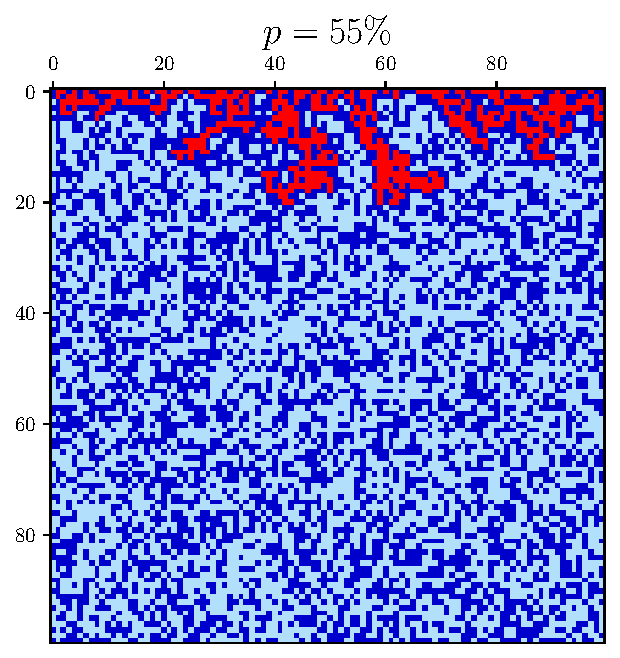
\includegraphics[width=\linewidth]{\pfig/dfs-55}
        \end{subfigure}
        \begin{subfigure}{0.45\linewidth}
            \centering
            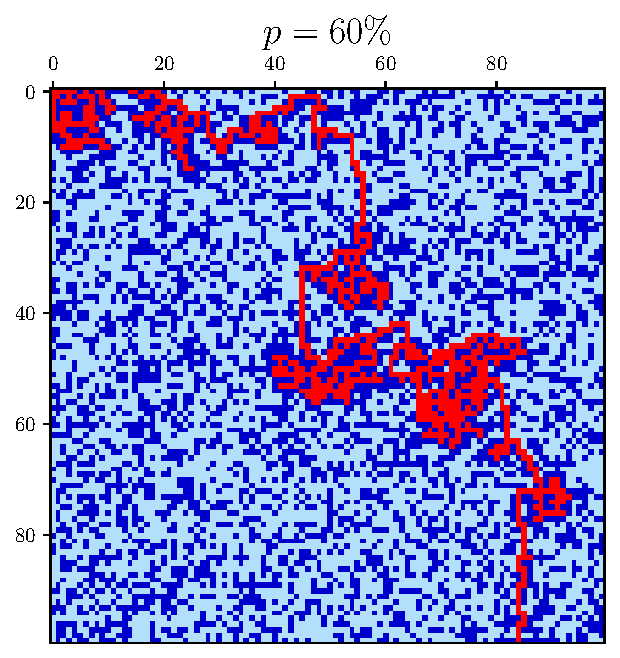
\includegraphics[width=\linewidth]{\pfig/dfs-60}
        \end{subfigure}
        \begin{subfigure}{0.45\linewidth}
            \centering
            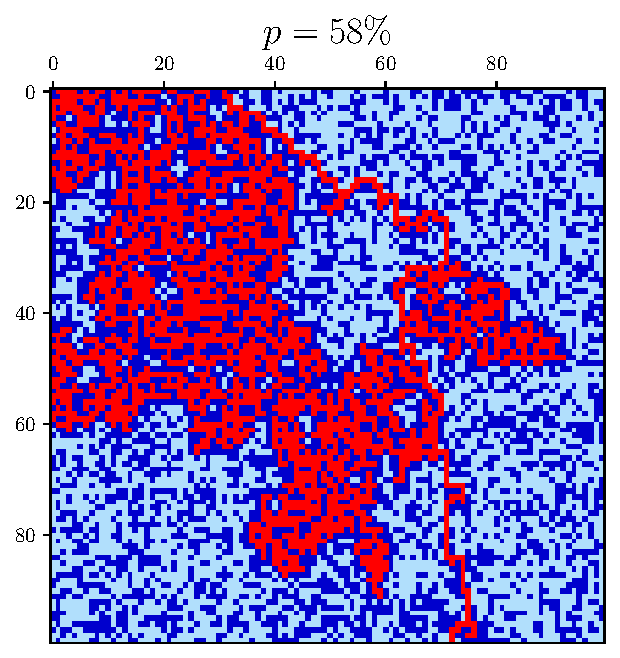
\includegraphics[width=\linewidth]{\pfig/dfs-58}
        \end{subfigure}
    \end{figure}
    \restoregeometry
    \subsection{Coloring}
    We can use (a very inefficient\footnote{$\mathcal{O}(L^{2d})$ time complexity}) coloring algorithm, as described in
    the lecture notes, to label the clusters in the grid. Then, If a cluster connecting the two ends of the grid exists,
    percolation is possible.
    \begin{figure}
        \centering
        \begin{subfigure}{0.45\linewidth}
            \centering
            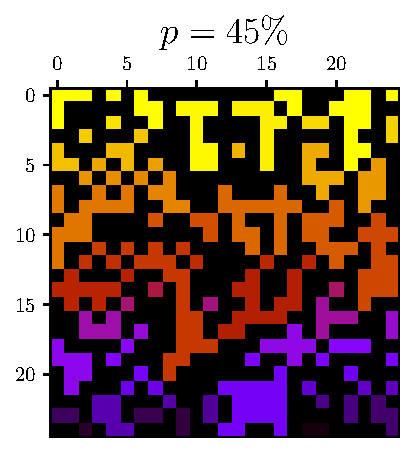
\includegraphics[width=\linewidth]{\pfig/color-45}
        \end{subfigure}
        \begin{subfigure}{0.45\linewidth}
            \centering
            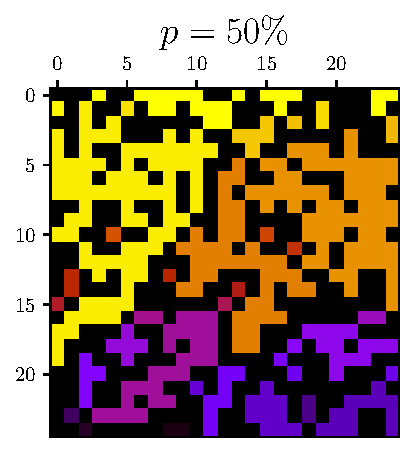
\includegraphics[width=\linewidth]{\pfig/color-50}
        \end{subfigure}
        \begin{subfigure}{0.45\linewidth}
            \centering
            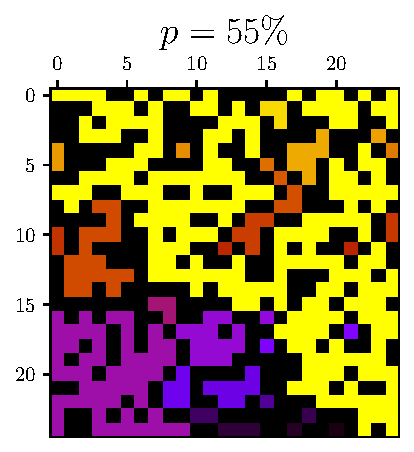
\includegraphics[width=\linewidth]{\pfig/color-55}
        \end{subfigure}
        \begin{subfigure}{0.45\linewidth}
            \centering
            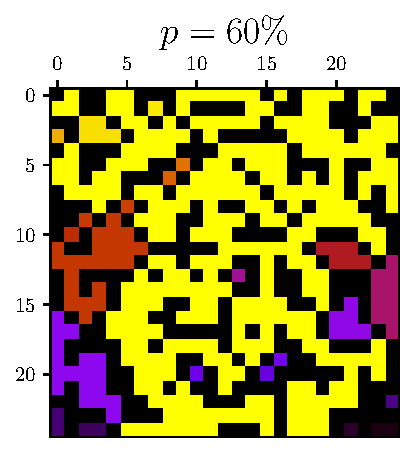
\includegraphics[width=\linewidth]{\pfig/color-60}
        \end{subfigure}
    \end{figure}
    \subsection{Hoshen--Kopelman}
    This is a much more efficient $\mathcal{O}(L^d)$ algorithm for labeling the clusters. You can read more about it
    on the \href{https://en.wikipedia.org/wiki/Hoshen%E2%80%93Kopelman_algorithm}{Wikipedia page}.
    \newgeometry{top=0.3in, bottom=0.3in, left=1in, right=1in}
    \thispagestyle{empty}
    \begin{figure}
        \centering
        \begin{subfigure}{\linewidth}
            \centering
            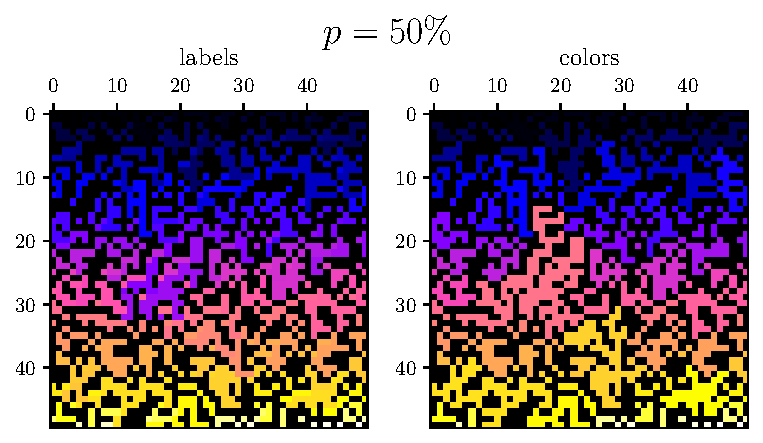
\includegraphics[width=\linewidth]{\pfig/hk-50}
        \end{subfigure}
        \begin{subfigure}{\linewidth}
            \centering
            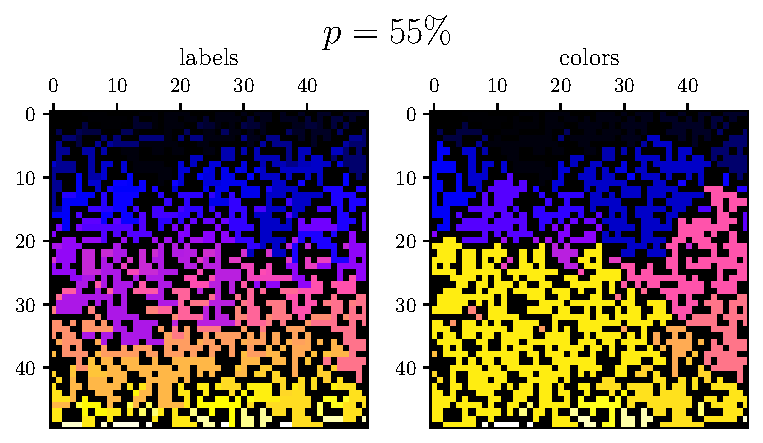
\includegraphics[width=\linewidth]{\pfig/hk-55}
        \end{subfigure}
        \begin{subfigure}{\linewidth}
            \centering
            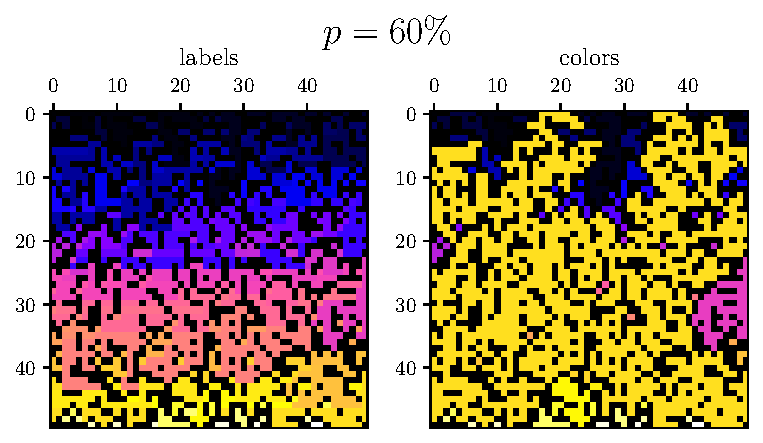
\includegraphics[width=\linewidth]{\pfig/hk-60}
        \end{subfigure}
    \end{figure}
    \restoregeometry
    \subsubsection{Percolation Probability}
    The probablity of there existing a path from the top to the bottom of a lattice (denoted by $Q$) exhibits critical
    behavior; If $p$ is the probablity of forming bonds (or sites) in the lattice, then is a sudden jump from 0 to 1
    probablity at a critical probablity $p_c$. In an infinite lattice, the path connecting the top and bottom of
    the lattice is called the \emph{infinite open cluster}.

    \begin{figure}
        \centering
        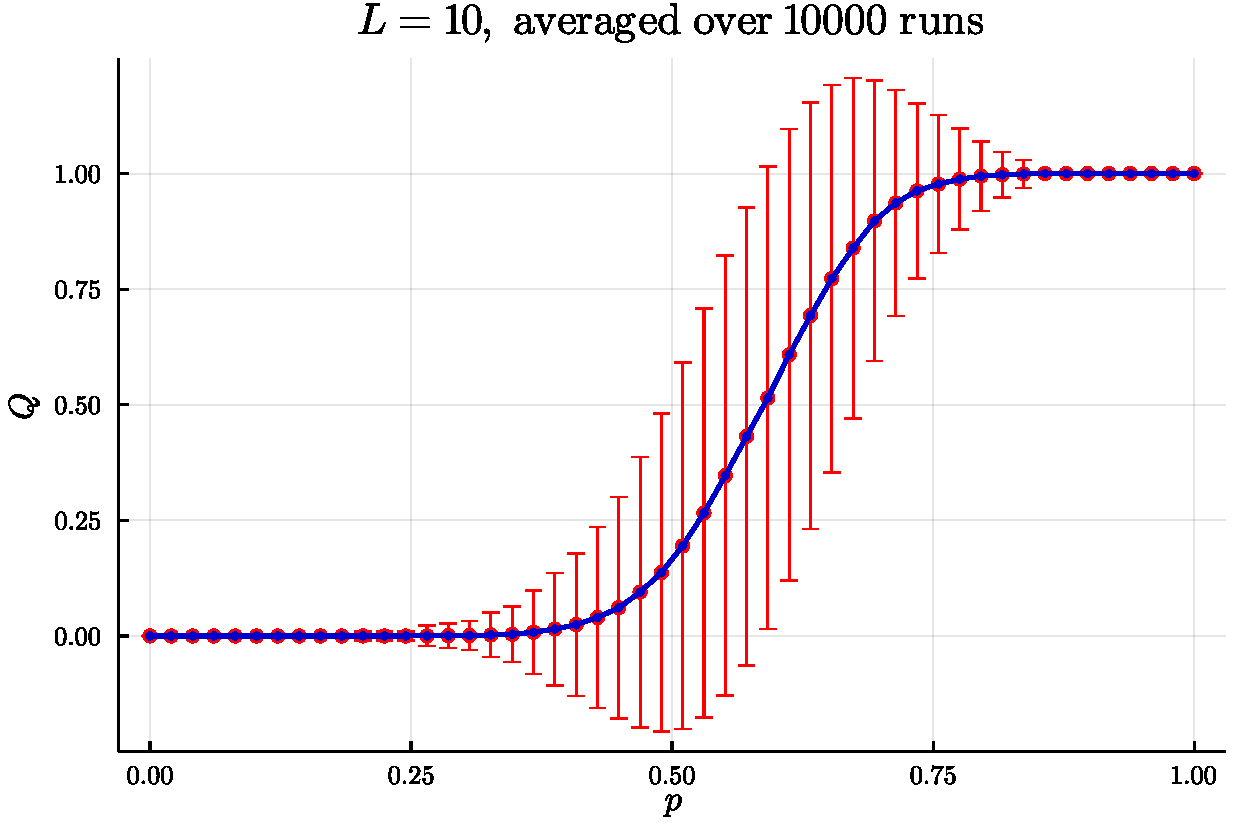
\includegraphics[width=\linewidth]{\pfig/percolate-full-10}
    \end{figure}
    \begin{figure}
        \centering
        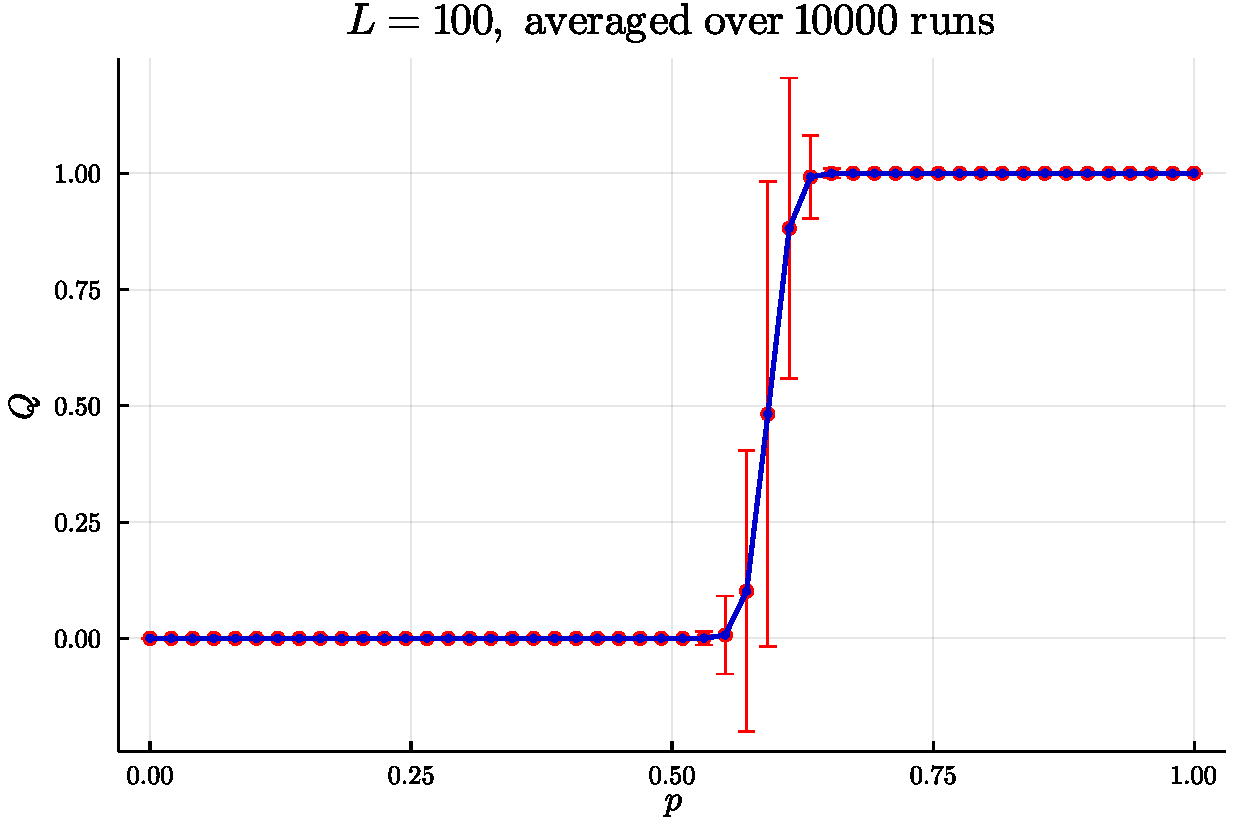
\includegraphics[width=\linewidth]{\pfig/percolate-full-100}
    \end{figure}
    \begin{figure}
        \centering
        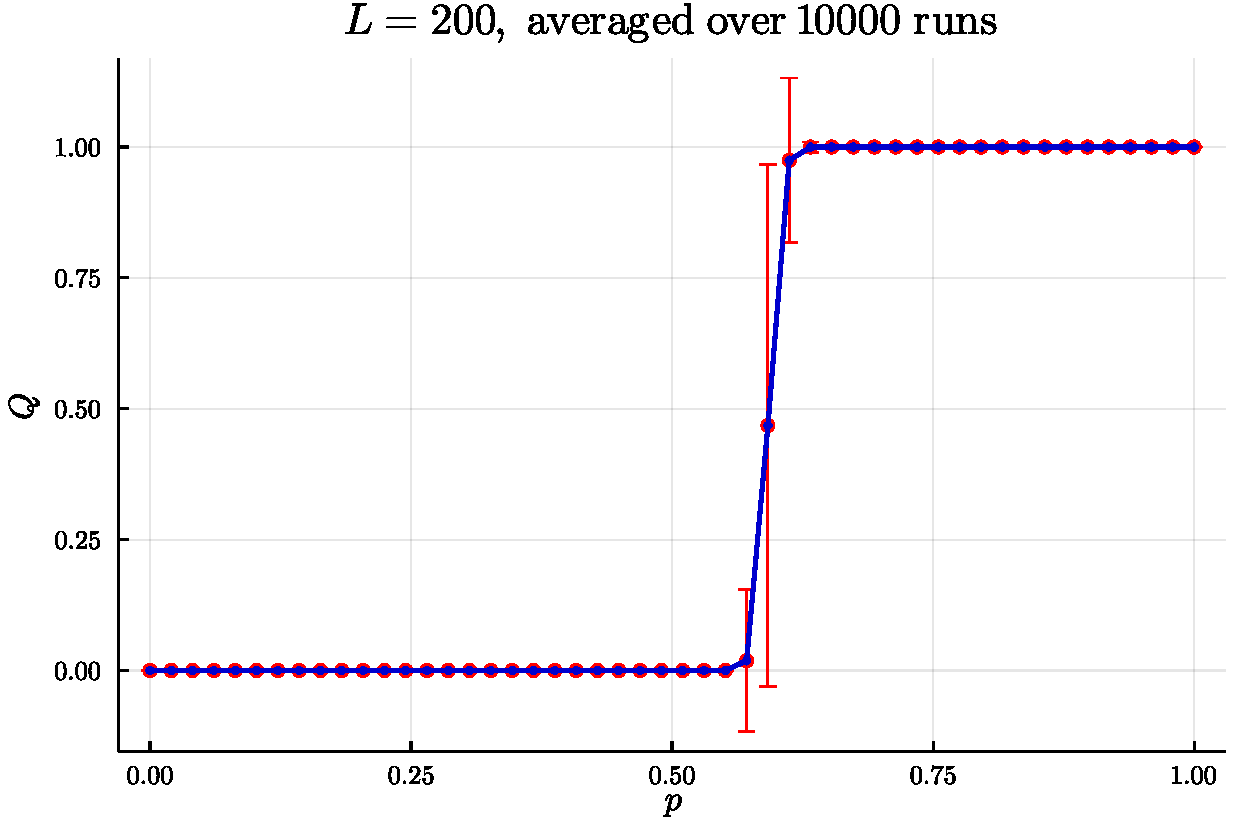
\includegraphics[width=\linewidth]{\pfig/percolate-full-200}
    \end{figure}
    \begin{figure}
        \centering
        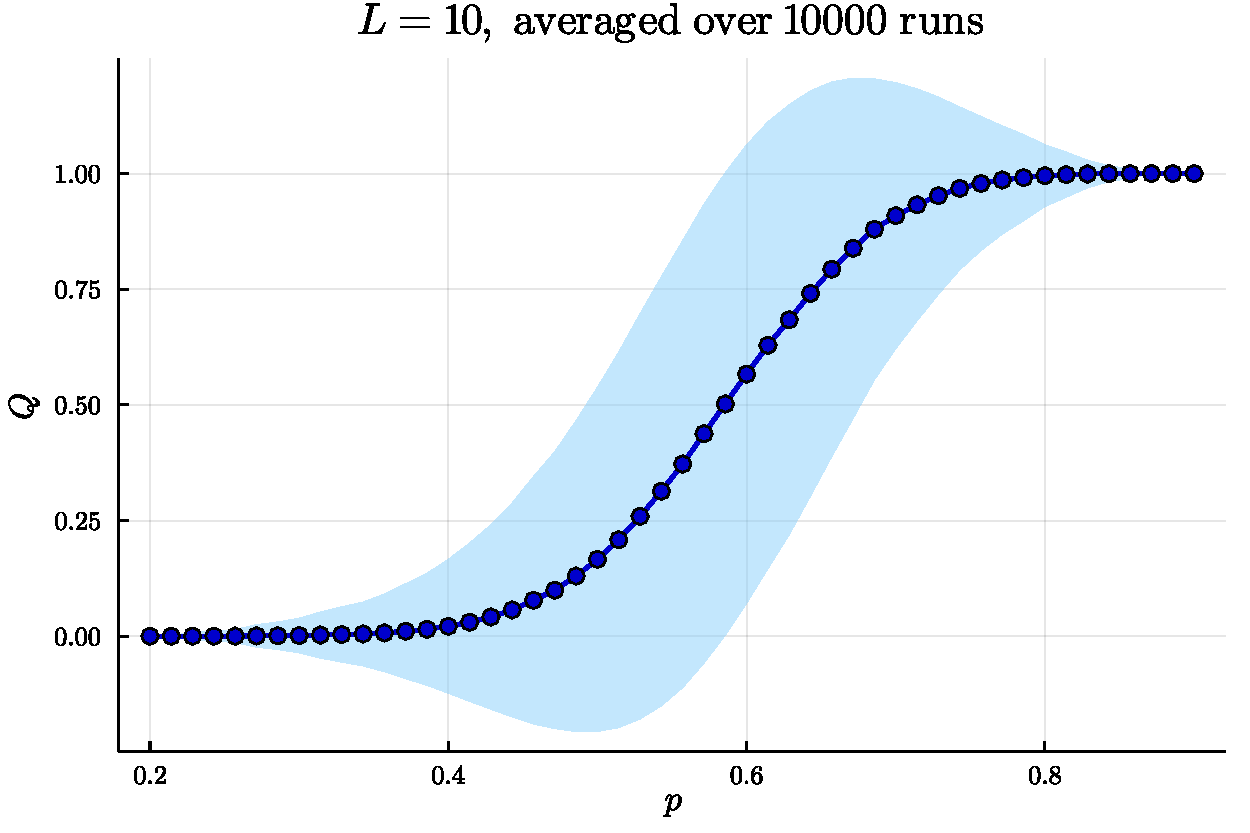
\includegraphics[width=\linewidth]{\pfig/percolate-zoom-10}
    \end{figure}
    \begin{figure}
        \centering
        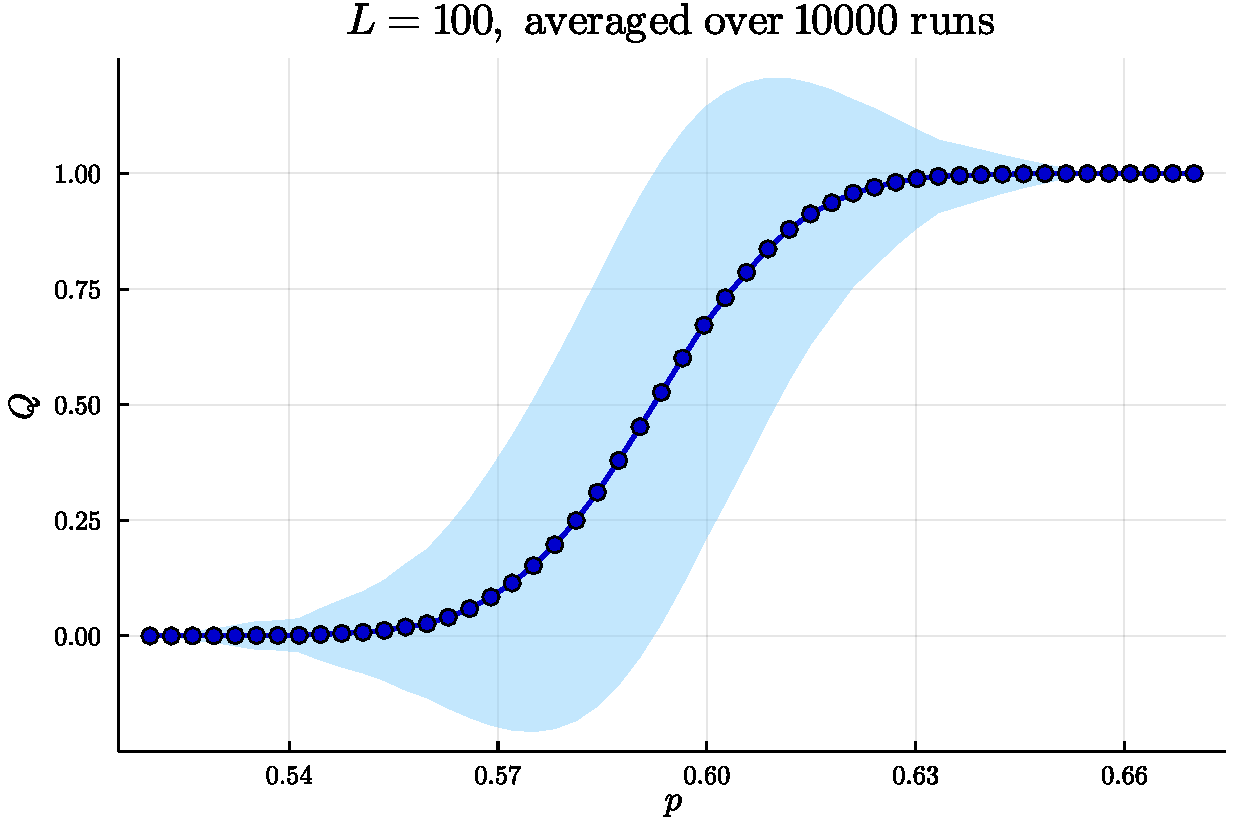
\includegraphics[width=\linewidth]{\pfig/percolate-zoom-100}
    \end{figure}
    \begin{figure}
        \centering
        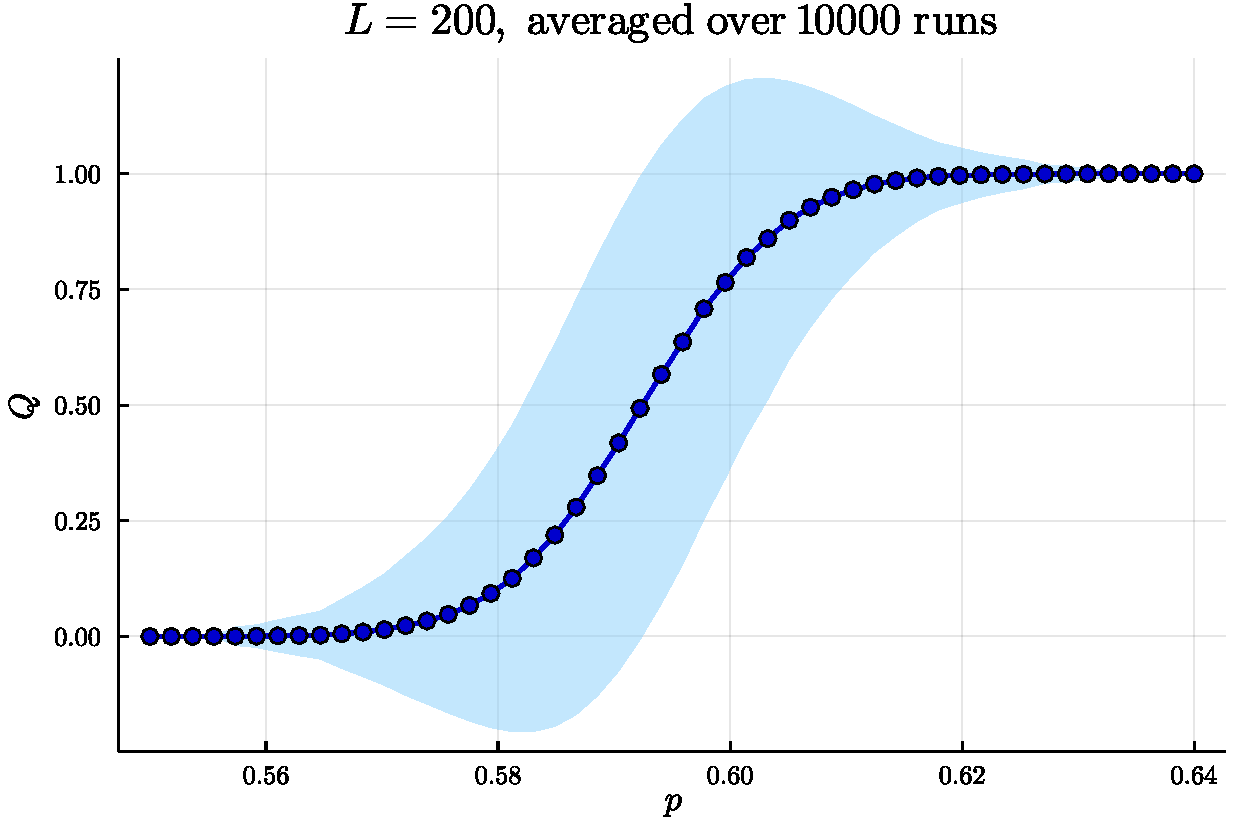
\includegraphics[width=\linewidth]{\pfig/percolate-zoom-200}
    \end{figure}

    As you can see, the transition from 0 to 1 probablity at $p_c$ becomes sharper as the side-length of the lattice
    increases.

    We use $Q_\infty$ to denote the probablity of a cell being a part of an open cluster connecting the top and bottom
    of the lattice. To calculate $Q_\infty$, we can modify the Hoshen--Kopelman algorithm to record cluster sizes for
    every label (that is, the "root" labels, or the final label that the cluster is connected to, such that
    $\mathrm{Label(number) = number}$). Then, $Q_\infty$ will be the sum of the sizes of the open clusters devided by
    the surface area of the lattice.

    \begin{figure}
        \centering
        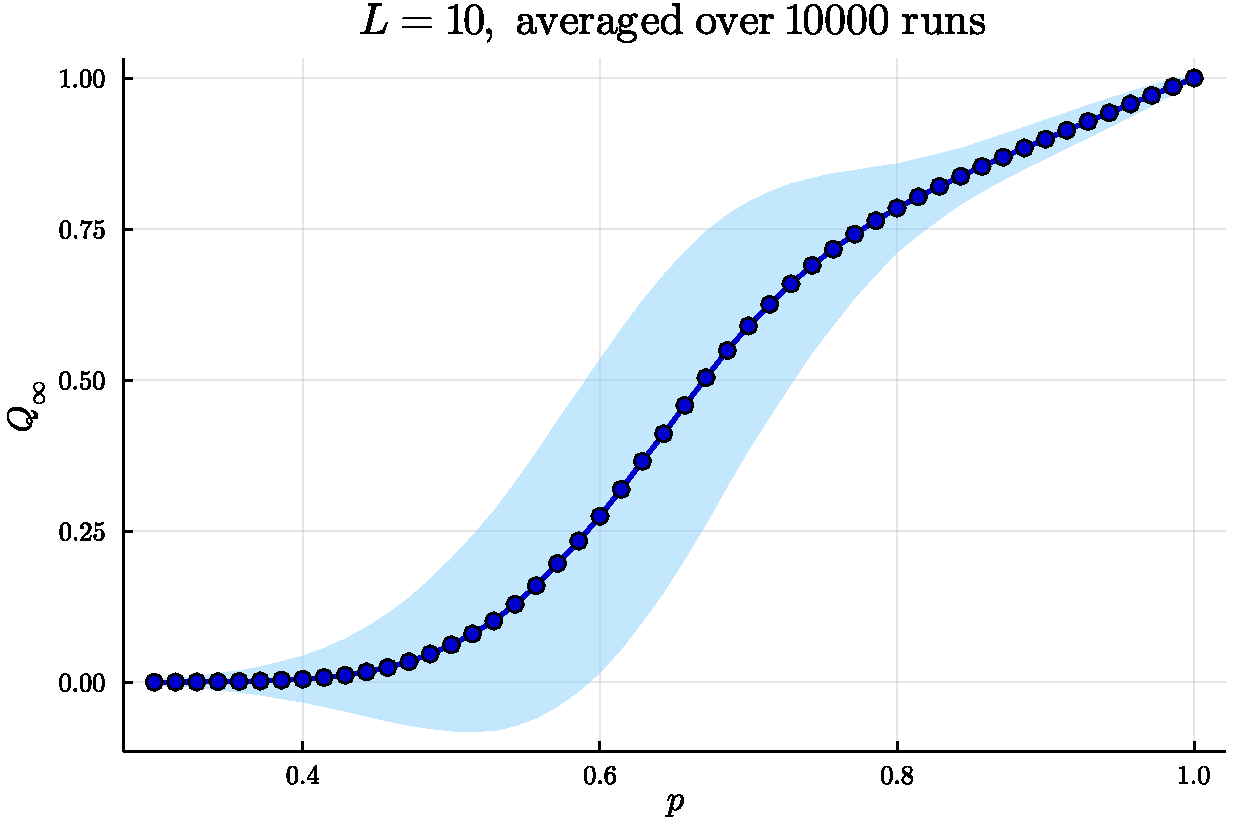
\includegraphics[width=\linewidth]{\pfig/percolate-qinfty-10}
    \end{figure}
    \begin{figure}
        \centering
        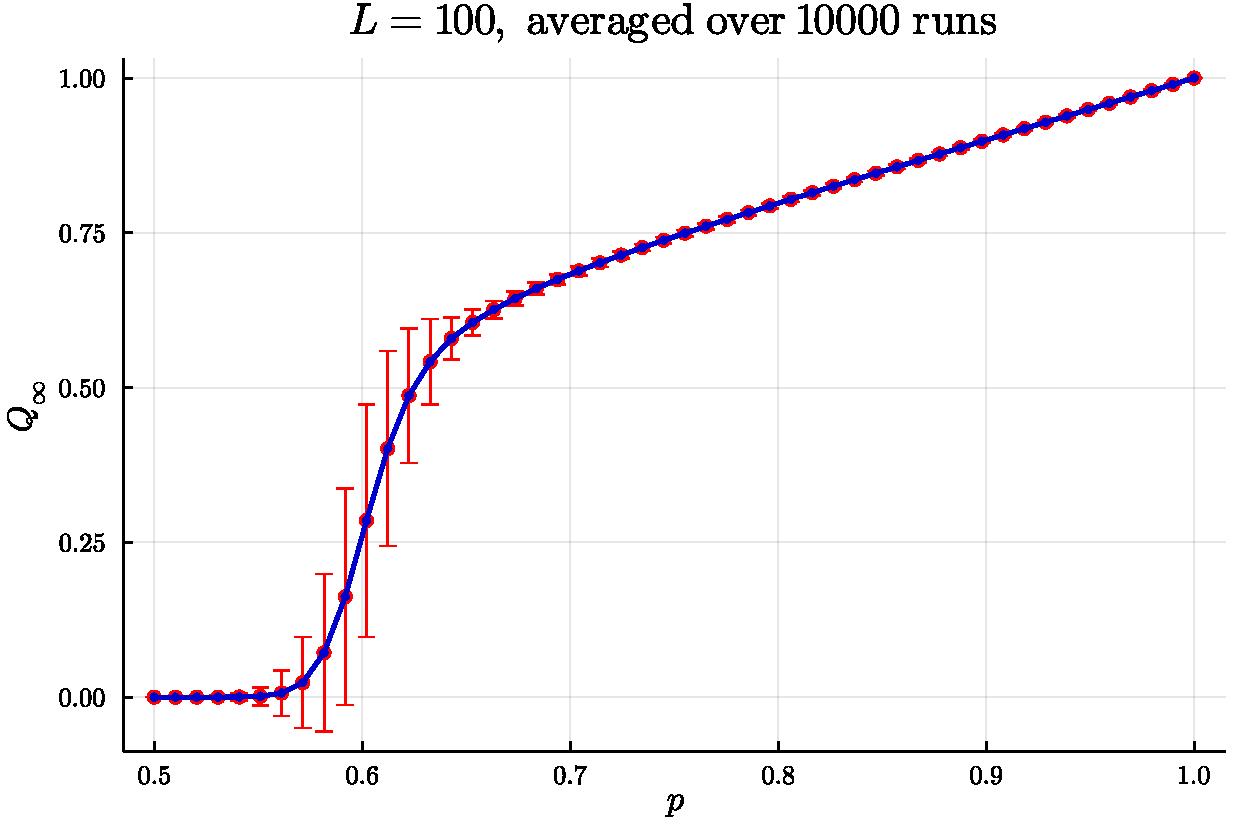
\includegraphics[width=\linewidth]{\pfig/percolate-qinfty-100}
    \end{figure}

    As you can see, $Q_\infty$ exhibits the same critical behavior as $Q$.
\end{document}
